\chapter{Results and Discussion}\label{ch:04results_discussion}
%TODO Remove chapter summary?

This chapter presents the results of the experiments as performed according to the plan described in Chapter~\ref{ch:03methods}. Section~\ref{results} provides the data and these results are discussed in more detail in Section~\ref{discussion}. 

\section{Results}\label{results}
In this section, the results of the experiments are presented. For each examined aspect, both a graphical representation of the data and some of the statistics are given, beginning with the conditions' impact on genome size. It should be noted that in many of the figures throughout this chapter, a rolling window of the mean was used to smooth the values, resulting in many of the plots only showing data starting after a few thousand generations (typically 10,000). This is simply an artifact of the graphing process, and simulations were indeed carried out for 500,000 generations. Lastly, since Aevol provides statistics for both the best individual at the end of the generation as well as for the population at large, the values given in the tables and graphs are for the population at large unless specified as being for the best individual. 

\subsection{Genome Size}\label{sec:genome_size}

In this section the results of the different conditions are examined, beginning with a focus on which, if any, lead to a reduced genome. Figure~\ref{fig:genome_size} presents the main findings regarding genome size. In the figure, the blue line shows the control condition and the other colors show the changed conditions: $\mu_+$/$\mu_-$ (mutation up/down), $k_+$/$k_-$ (selection up/down), and $N_+$/$N_-$ (population up/down). As can be seen from the figure, the expectations from Section~\ref{sec:expected_results} did not always hold up, as several conditions actually \textit{increased} over their original size. 
\begin{figure}[H]
	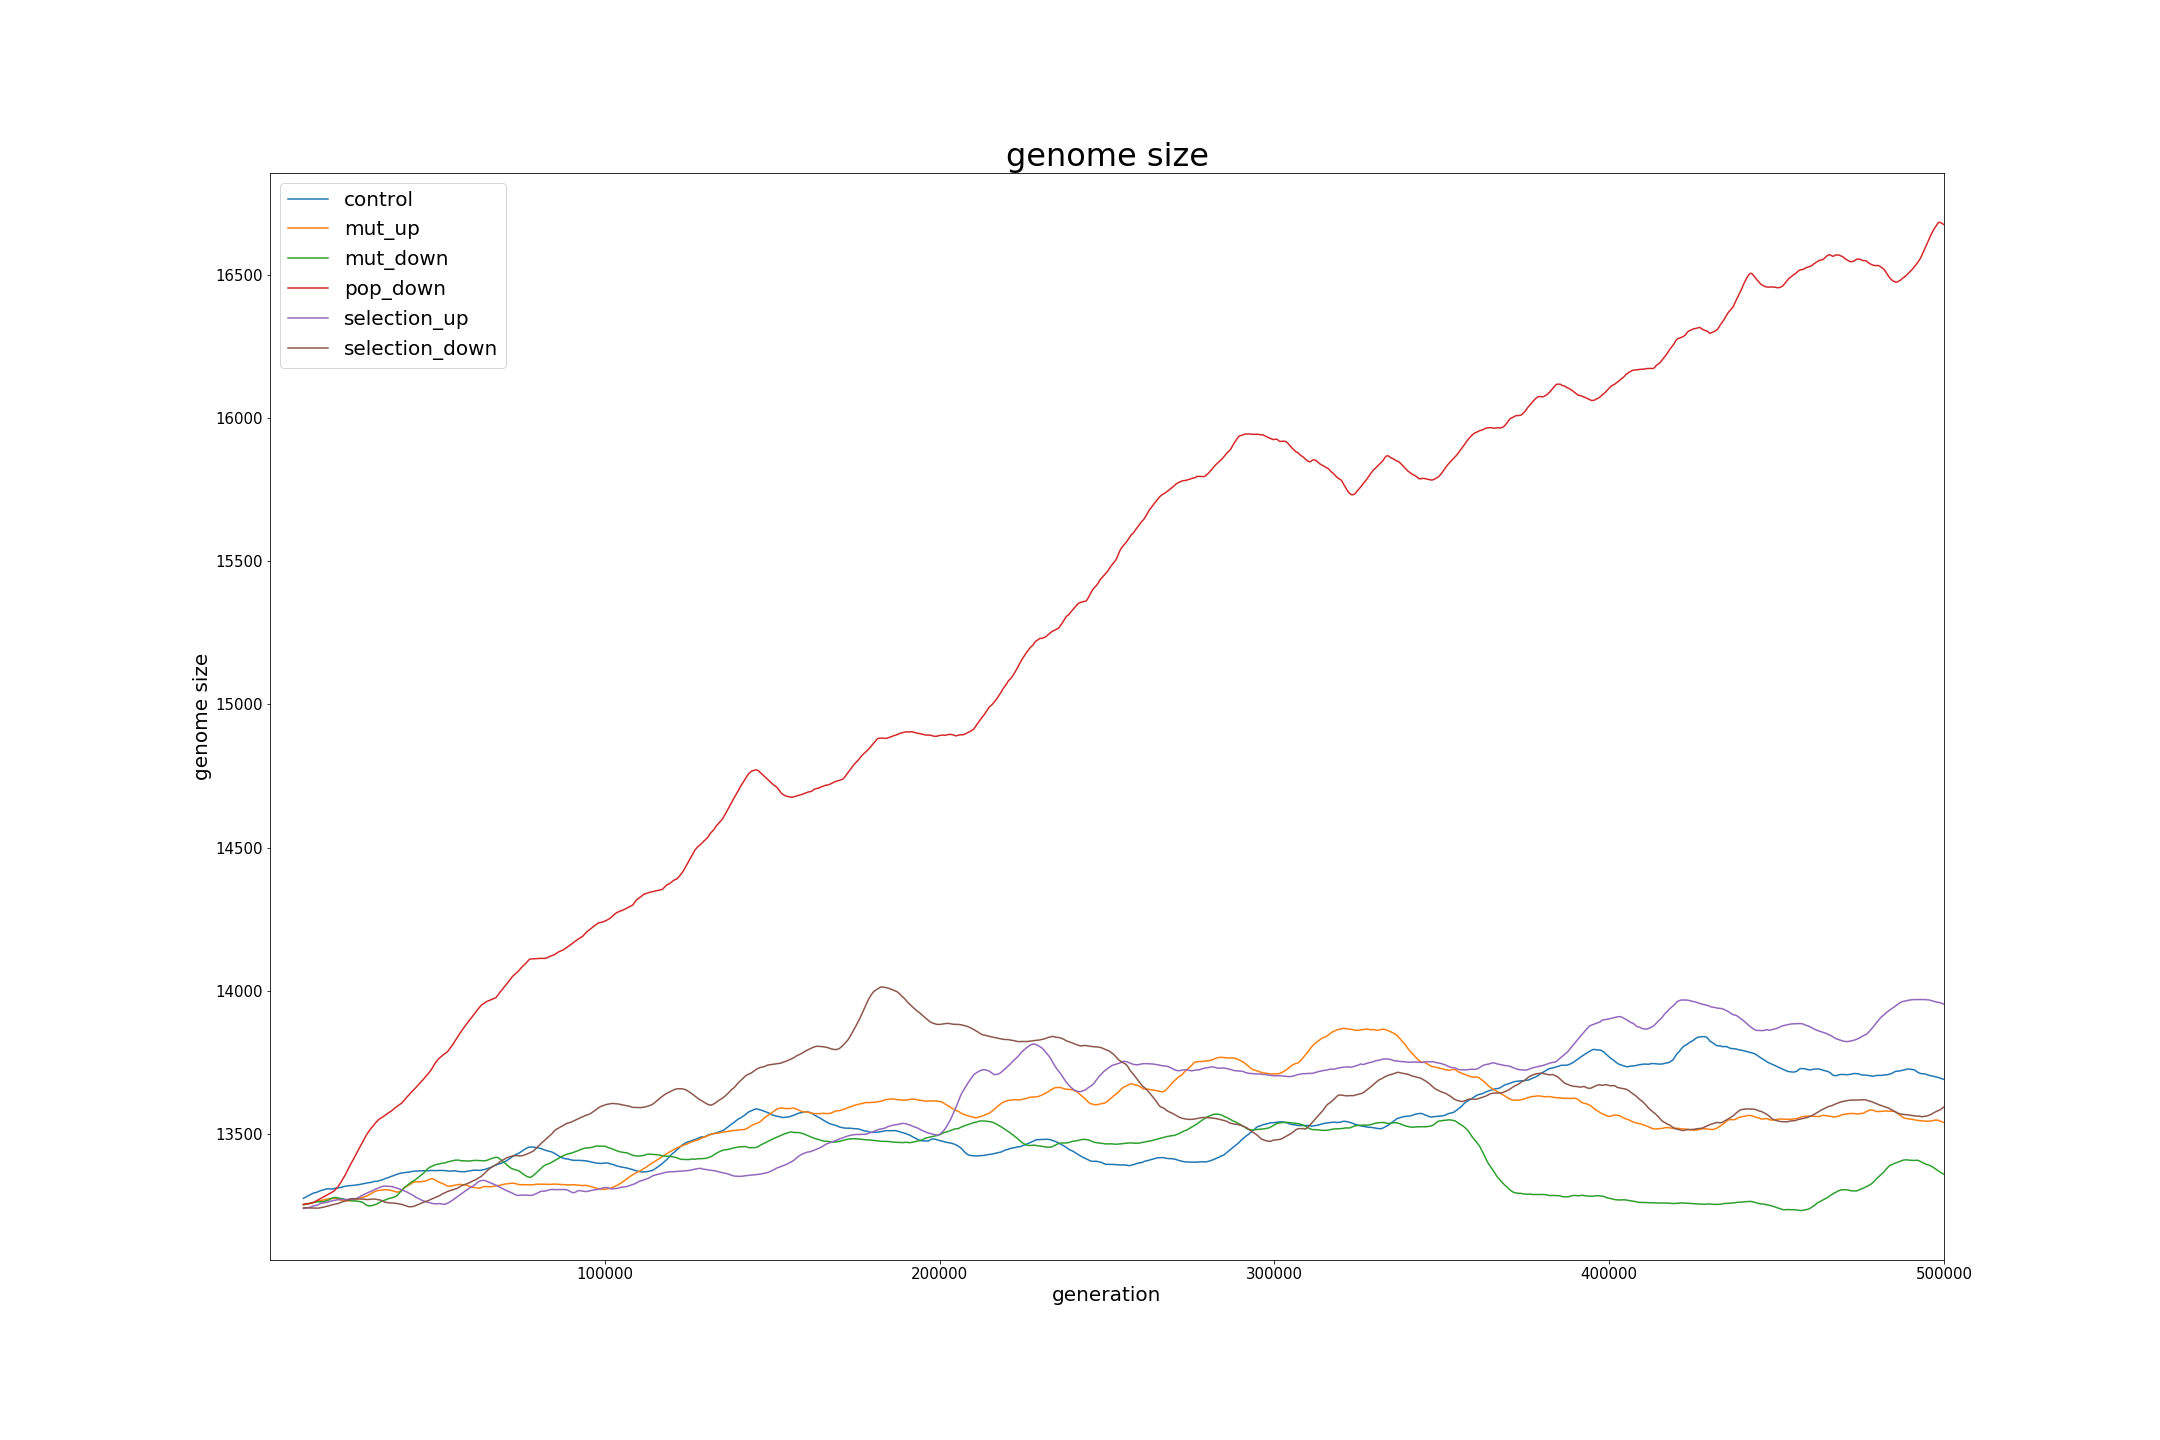
\includegraphics[width=\linewidth]{stat_fitness_global_mean_genome_size}
	\centering
	\caption[Genome size]{Average genome size across the population, in number of bases, of all conditions. Average taken across all five seeds for each condition.}
	\label{fig:genome_size}
\end{figure}
In fact, the $N_-$ condition had a runaway increase in the number of bases, reaching over 16,500 bases at one time, a 25\% increase over the original wild type's roughly 13,200 bp. Even after 500,000 generations, it seems that the upper size limit may still not have been reached. The statistical results are given below in Tables~\ref{table:genome_size_stats} and \ref{table:genome_size_mean_and_std_dev}, which show the mean and standard deviation for all seeds across all 500,000 generations. 

\begin{table}[H]
	\begin{tabular}{|c|c|c|c|}
		\hline
		\multicolumn{4}{c}{\Large \textbf{Genome Size - 500k Gen. Mean \& Std. Dev. (in bp)}} \\
		\hline
		 & \textbf{mean} & \textbf{standard deviation} & \textbf{mean's \% change from control} \\
		 \hline
		 control & 13537.031513 & 144.351138 & \textemdash \\ 
		 \hline
		 $\mu_+$ & 13558.374160 & 155.077847 & 0.157661 \\ 
		 \hline
		 $\mu_-$ & 13410.743690 & 101.376104 & -0.932906 \\ 
		 \hline
		 $k_+$ & 13621.901104 & 229.635708 & 0.626944 \\ 
		 \hline
		 $k_-$ & 13614.663599 & 172.675042 & 0.573479 \\ 
		 \hline
		 $N_-$ & 15275.149392 & 950.266243 & 12.839727 \\ 
		 \hline
	\end{tabular}
	\caption[Genome size - mean and std. dev.]{Average genome size across all 500,000 generations, with standard deviation for all seeds and all conditions. }
	\label{table:genome_size_mean_and_std_dev}
\end{table}

\begin{table}[H]
	\centering
	\begin{tabular}{|c|c|c|}
		\hline
		\multicolumn{3}{c}{\Large Genome Size - Rank Sum \& P-Values} \\
		\hline
		& \textbf{rank sum U} & \textbf{p-value} \\
		\hline \hline
		$\mu_+$ & 110508011469.50 & 0.00000000 \\ 
		\hline
		$\mu_-$ & 71008638349.50 & 0.00000000 \\ 
		\hline
		$N_-$ & 16477791900.50 & 0.00000000 \\ 
		\hline
		$k_+$ & 100151680984.50 & 0.00000000 \\ 
		\hline
		$k_-$ & 88533681875.00 & 0.00000000 \\ 
		\hline
	\end{tabular}
	\caption[Genome size rank sum statistics]{Genome size rank sum statistics.}
	\label{table:genome_size_stats}
\end{table} 

Of the remaining conditions, all but the $k_+$ condition (which had an an increase of 11\% over the control condition) ended up with fewer base pairs than the control condition, though all increased slightly over their starting point. Also noteworthy is that the mutation down condition appears to have had a steady increase in the number of base pairs until a maximum of just over 14,000 around generation 350,000 before having a fairly sharp decline back to nearly the original size. 

Examining the percent changed from the \textit{control} condition shown in Figure~\ref{fig:genome_size_percent_change} it can be seen that at points, the $\mu_-$ condition was nearly 5\% smaller than the \textit{control} condition. 

\begin{figure}[H]
	\centering
	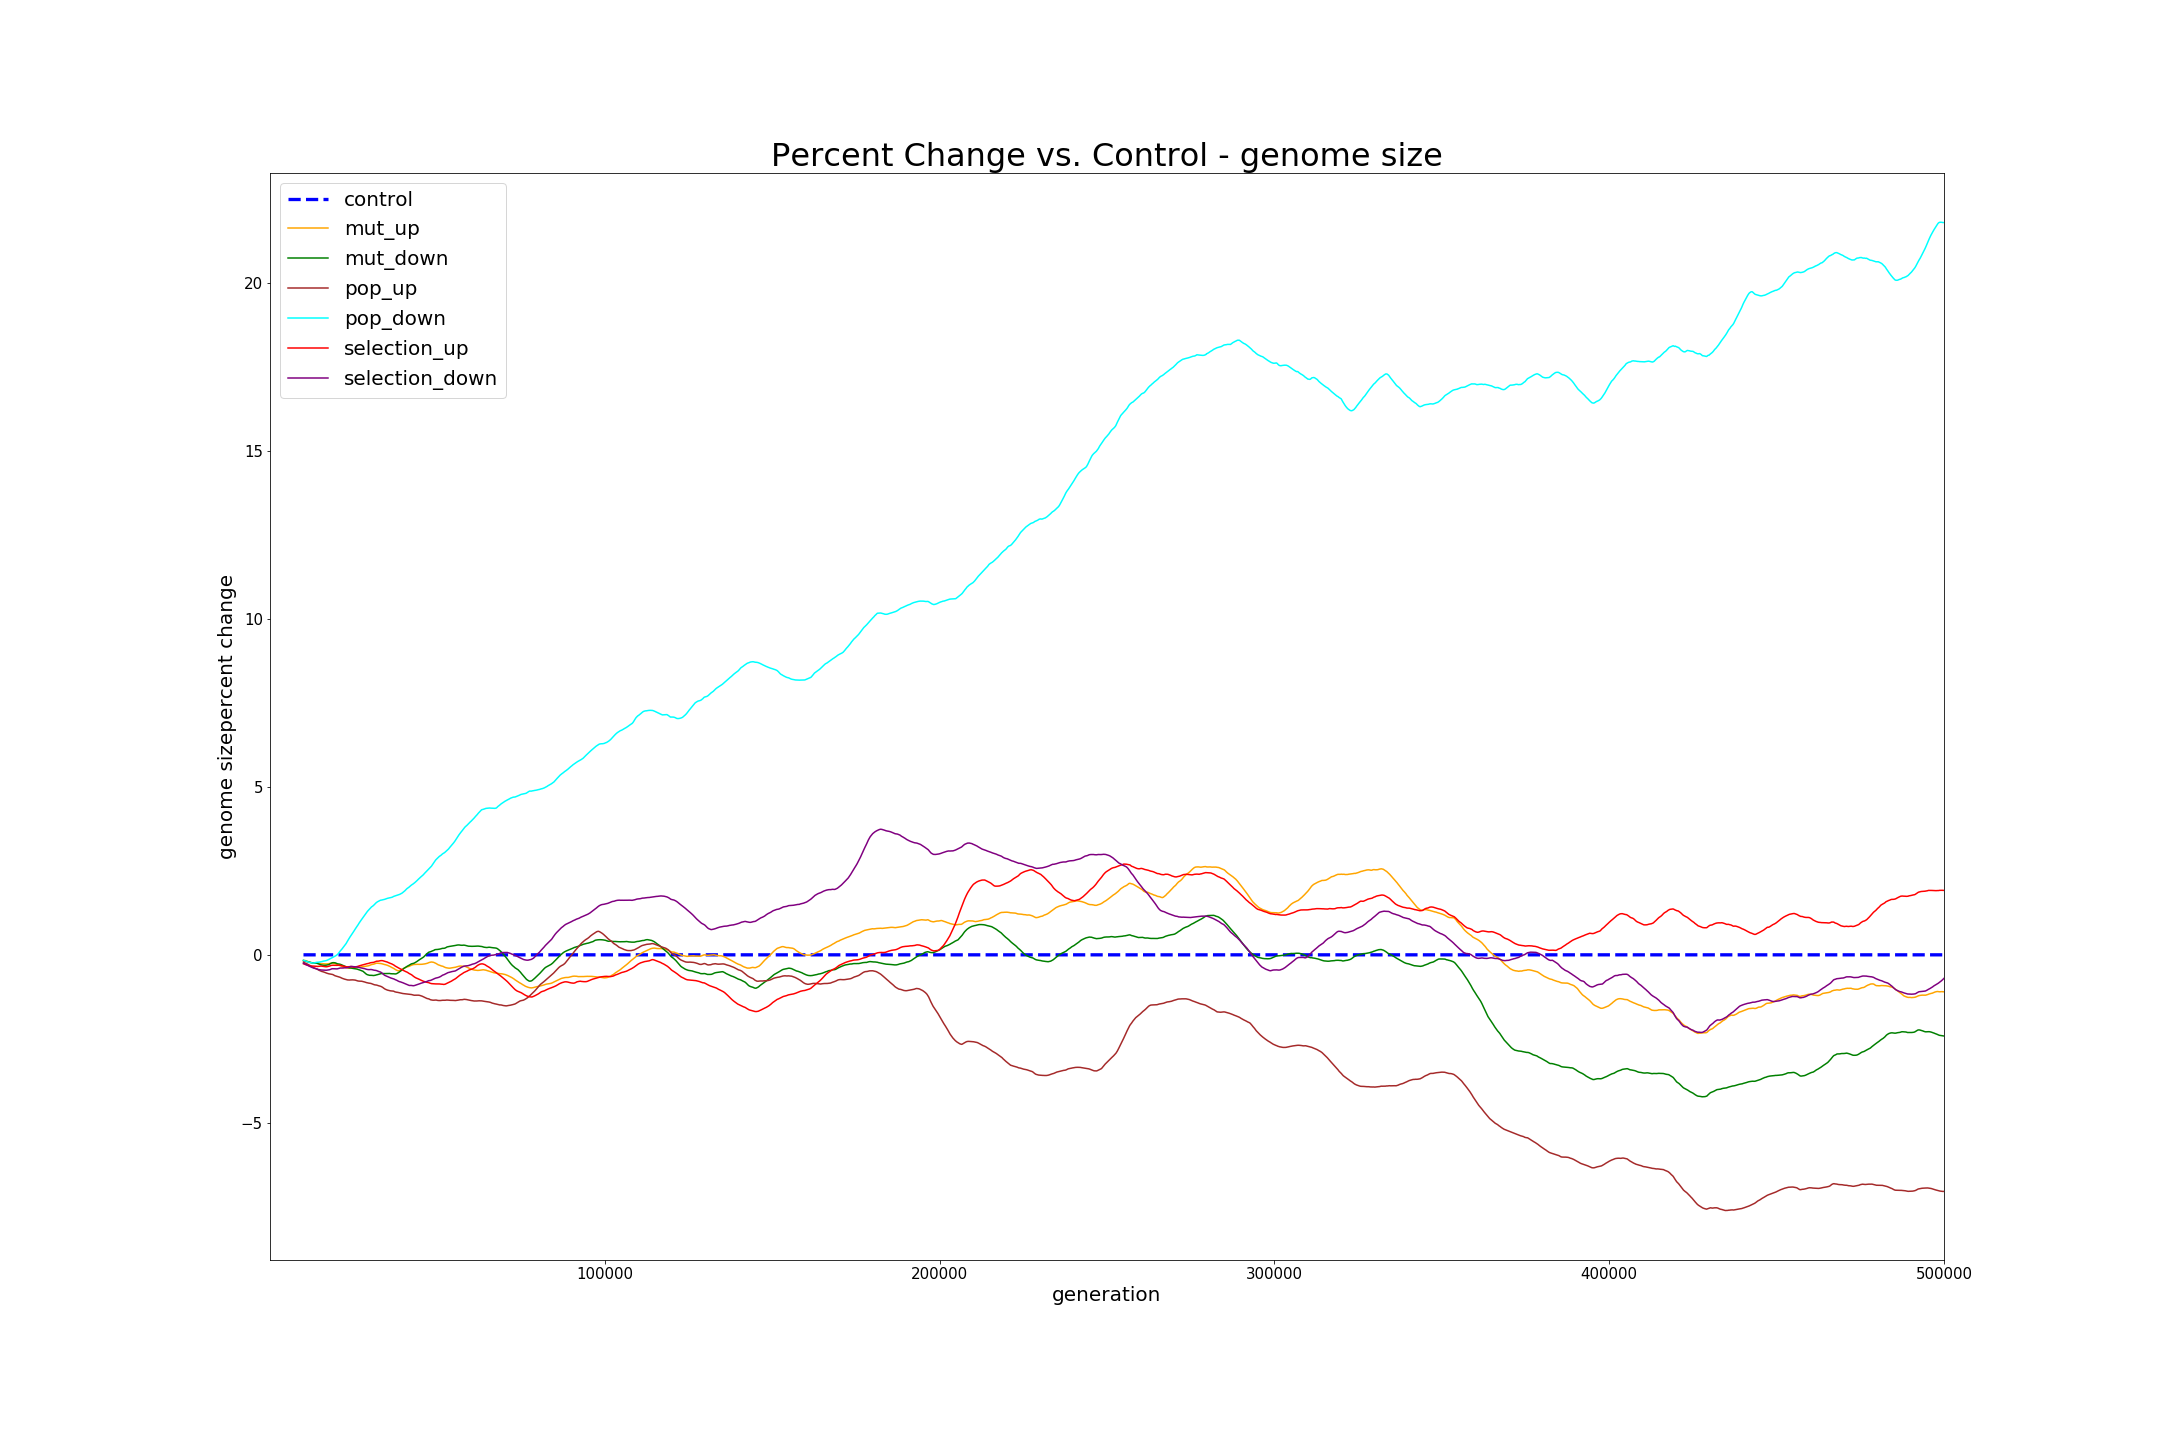
\includegraphics[width=\linewidth]{stat_fitness_perc_change_genome_size}
	\caption[Genome size - percent change]{Genome size's percent change from the \textit{control} condition.}
	\label{fig:genome_size_percent_change}
\end{figure}

Lastly, looking at just the last 50,000 generations in Figure~\ref{fig:genome_size_last_50k} and the respective statistics in Table~%TODO Create table
, it becomes clear that, with the exception of the $N_-$ condition, the genome sizes did not generally differ much across the conditions.
\begin{figure}[H]
	\centering
	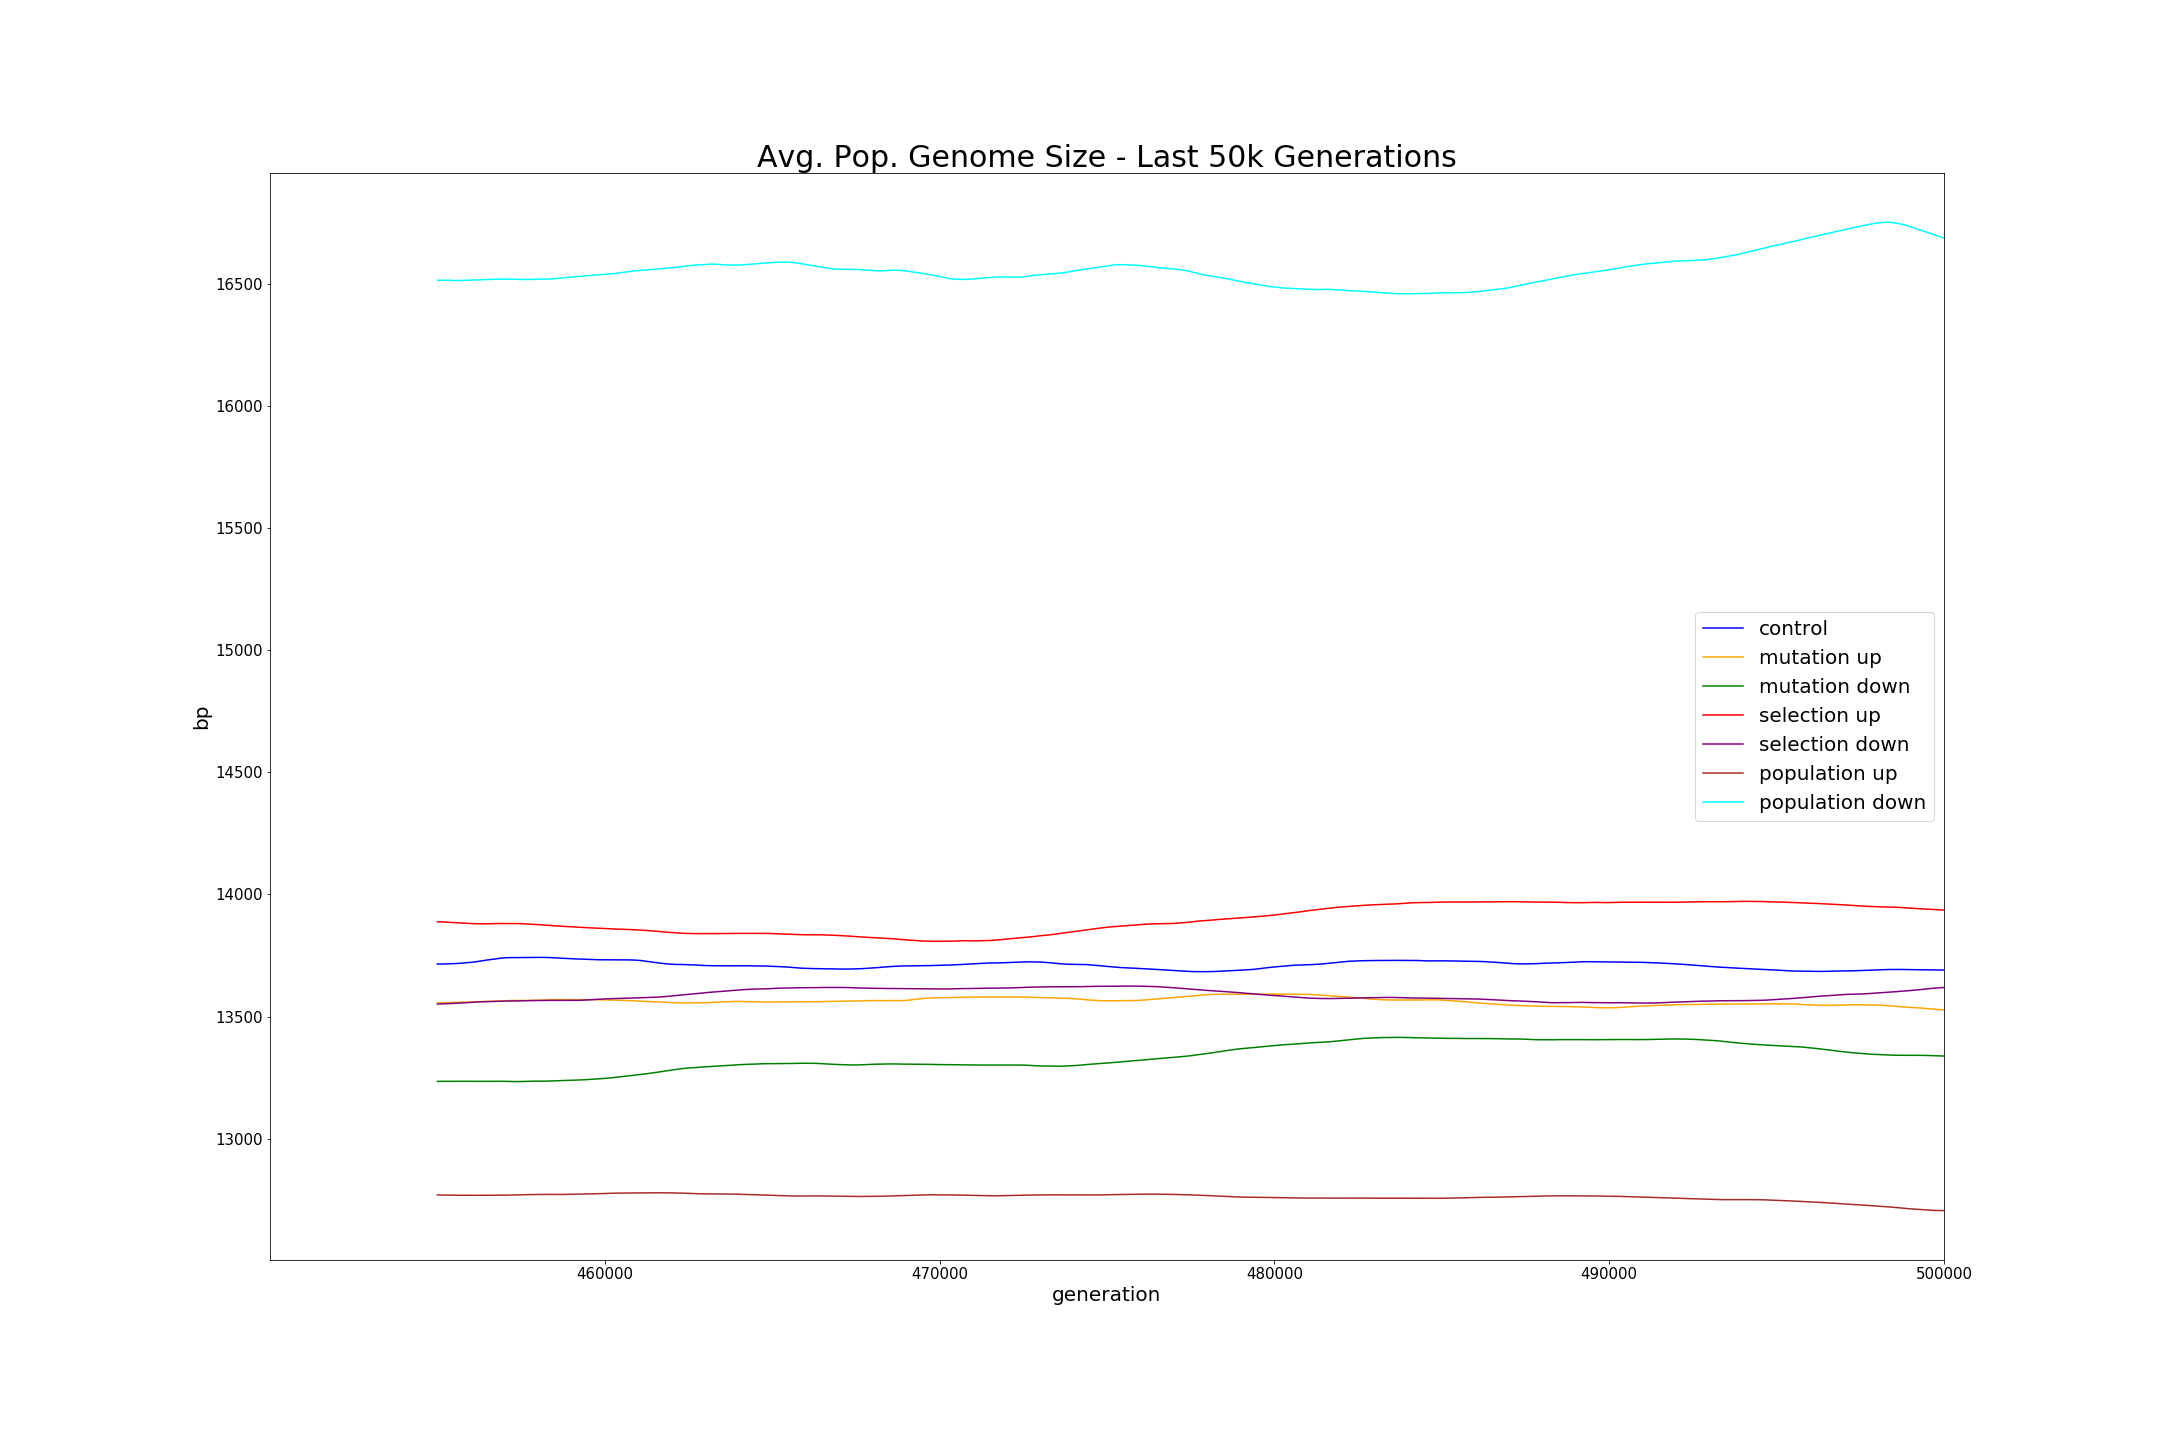
\includegraphics[width=\linewidth]{genome_size_last_50k}
	\caption[Genome size - last 50k generations]{Genome Size - Last 50k Generations, average of all seeds}
	\label{fig:genome_size_last_50k}
\end{figure}

\begin{table}[H]
	\begin{tabular}{|c|c|c|c|}
		\hline
		\multicolumn{4}{c}{\textbf{Genome Size - Last 50k Gen. Mean \& Std. Dev.}} \\
		\hline
		& \textbf{Mean} & \textbf{Std. Dev} & \textbf{\% change from control} \\
		\hline		
		\textbf{control} & \textbf{13711.33} & \textbf{15.7415} & \textemdash \\ 
		\hline
		$\mu_+$ & 13562.61 & 15.00505 & -1.084674 \\ 
		\hline
		$\mu_-$ & 13337.11 & 57.97296 & -2.729274\\ 
		\hline
		$k_+$ & 13900.82 & 58.01581 & 1.381967 \\ 
		\hline
		$k_-$ & 13588.36 & 23.64136 & -0.8968192 \\ 
		\hline
		$N_-$ & 16559.80 & 69.53241 & 20.77458 \\ 
		\hline
	\end{tabular}
	\caption[Genome size - last 50k generations mean \& std. dev.]{This table shows the mean, standard deviation, and percent change from the control condition for the population for just the last 50k generations.}
	\label{table:genome_size_stats_last_50k}
\end{table}


\subsection{Metabolic Error and Fitness}
%TODO Fix Metabolic Error and Fitness section
Figure~\ref{fig:mean_fitness_all_seeds} shows three categories of information for each condition: 1) the individual seeds for the population mean fitness for that seed (in various colors), 2) the mean fitness for all seeds for that condition (dashed line, black), 3) the control condition (dashed line, blue) for each condition. It is important to note that for the $k_+$ and $k_-$ conditions, the fitness is on a different scale because of the \texttt{fitness\_proportionate} selection method. Recall that in the \texttt{fitness\_proportionate} selection method, the probability $p$ of reproduction for an organism with gap $g$ is given by:
\begin{equation*}
p = \frac{e^{-k*g}}{\sum_{i=1}^{N}e^{-k*g_i}}
\end{equation*}
where $g_i$ is the gap for the $i$th organism in the population. Thus, changing the selection parameter $k$, as in the $k_+$ and $k_-$ conditions, changes the scale of the fitness values. Their behavior over time is more important than the scale, so they are nevertheless included in this set of plots. So as not to skew the scale of the plots, however, the control condition is left off of these plots. 

\begin{figure}[H]
	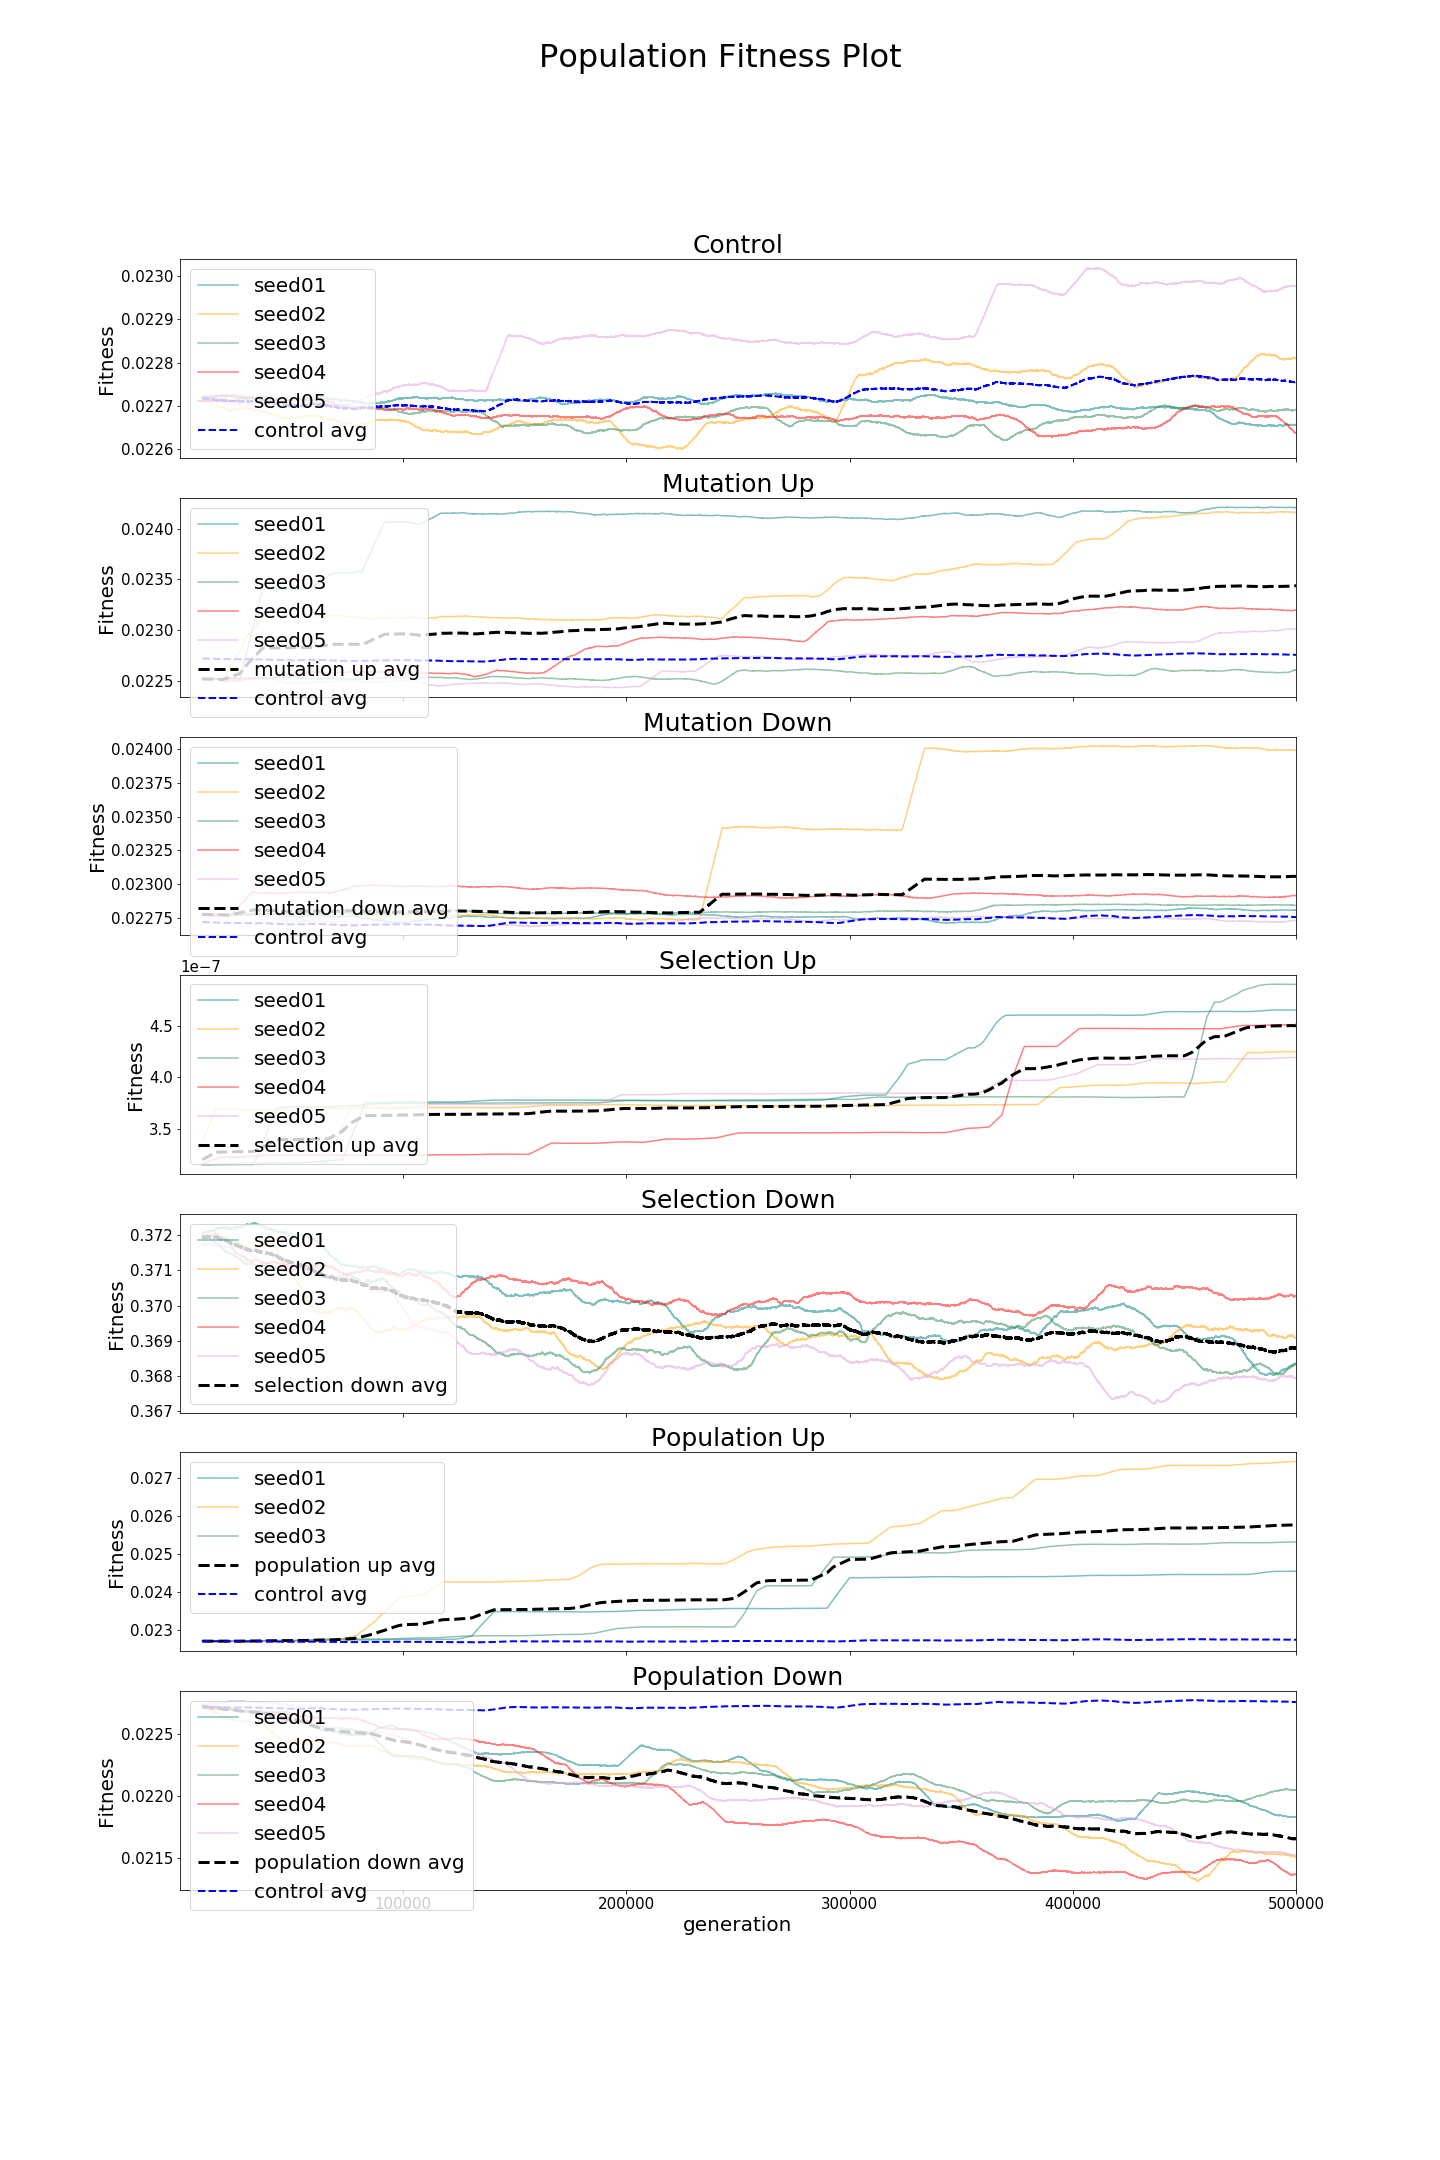
\includegraphics[width=\linewidth]{global_fitness_all_seeds}
	\caption[Fitness all seeds all conditions]{Mean population fitness for each condition. All seeds are shown; the average for that condition is shown in black and the control condition is blue.}
	\label{fig:mean_fitness_all_seeds}
\end{figure}

\begin{figure}[H]
	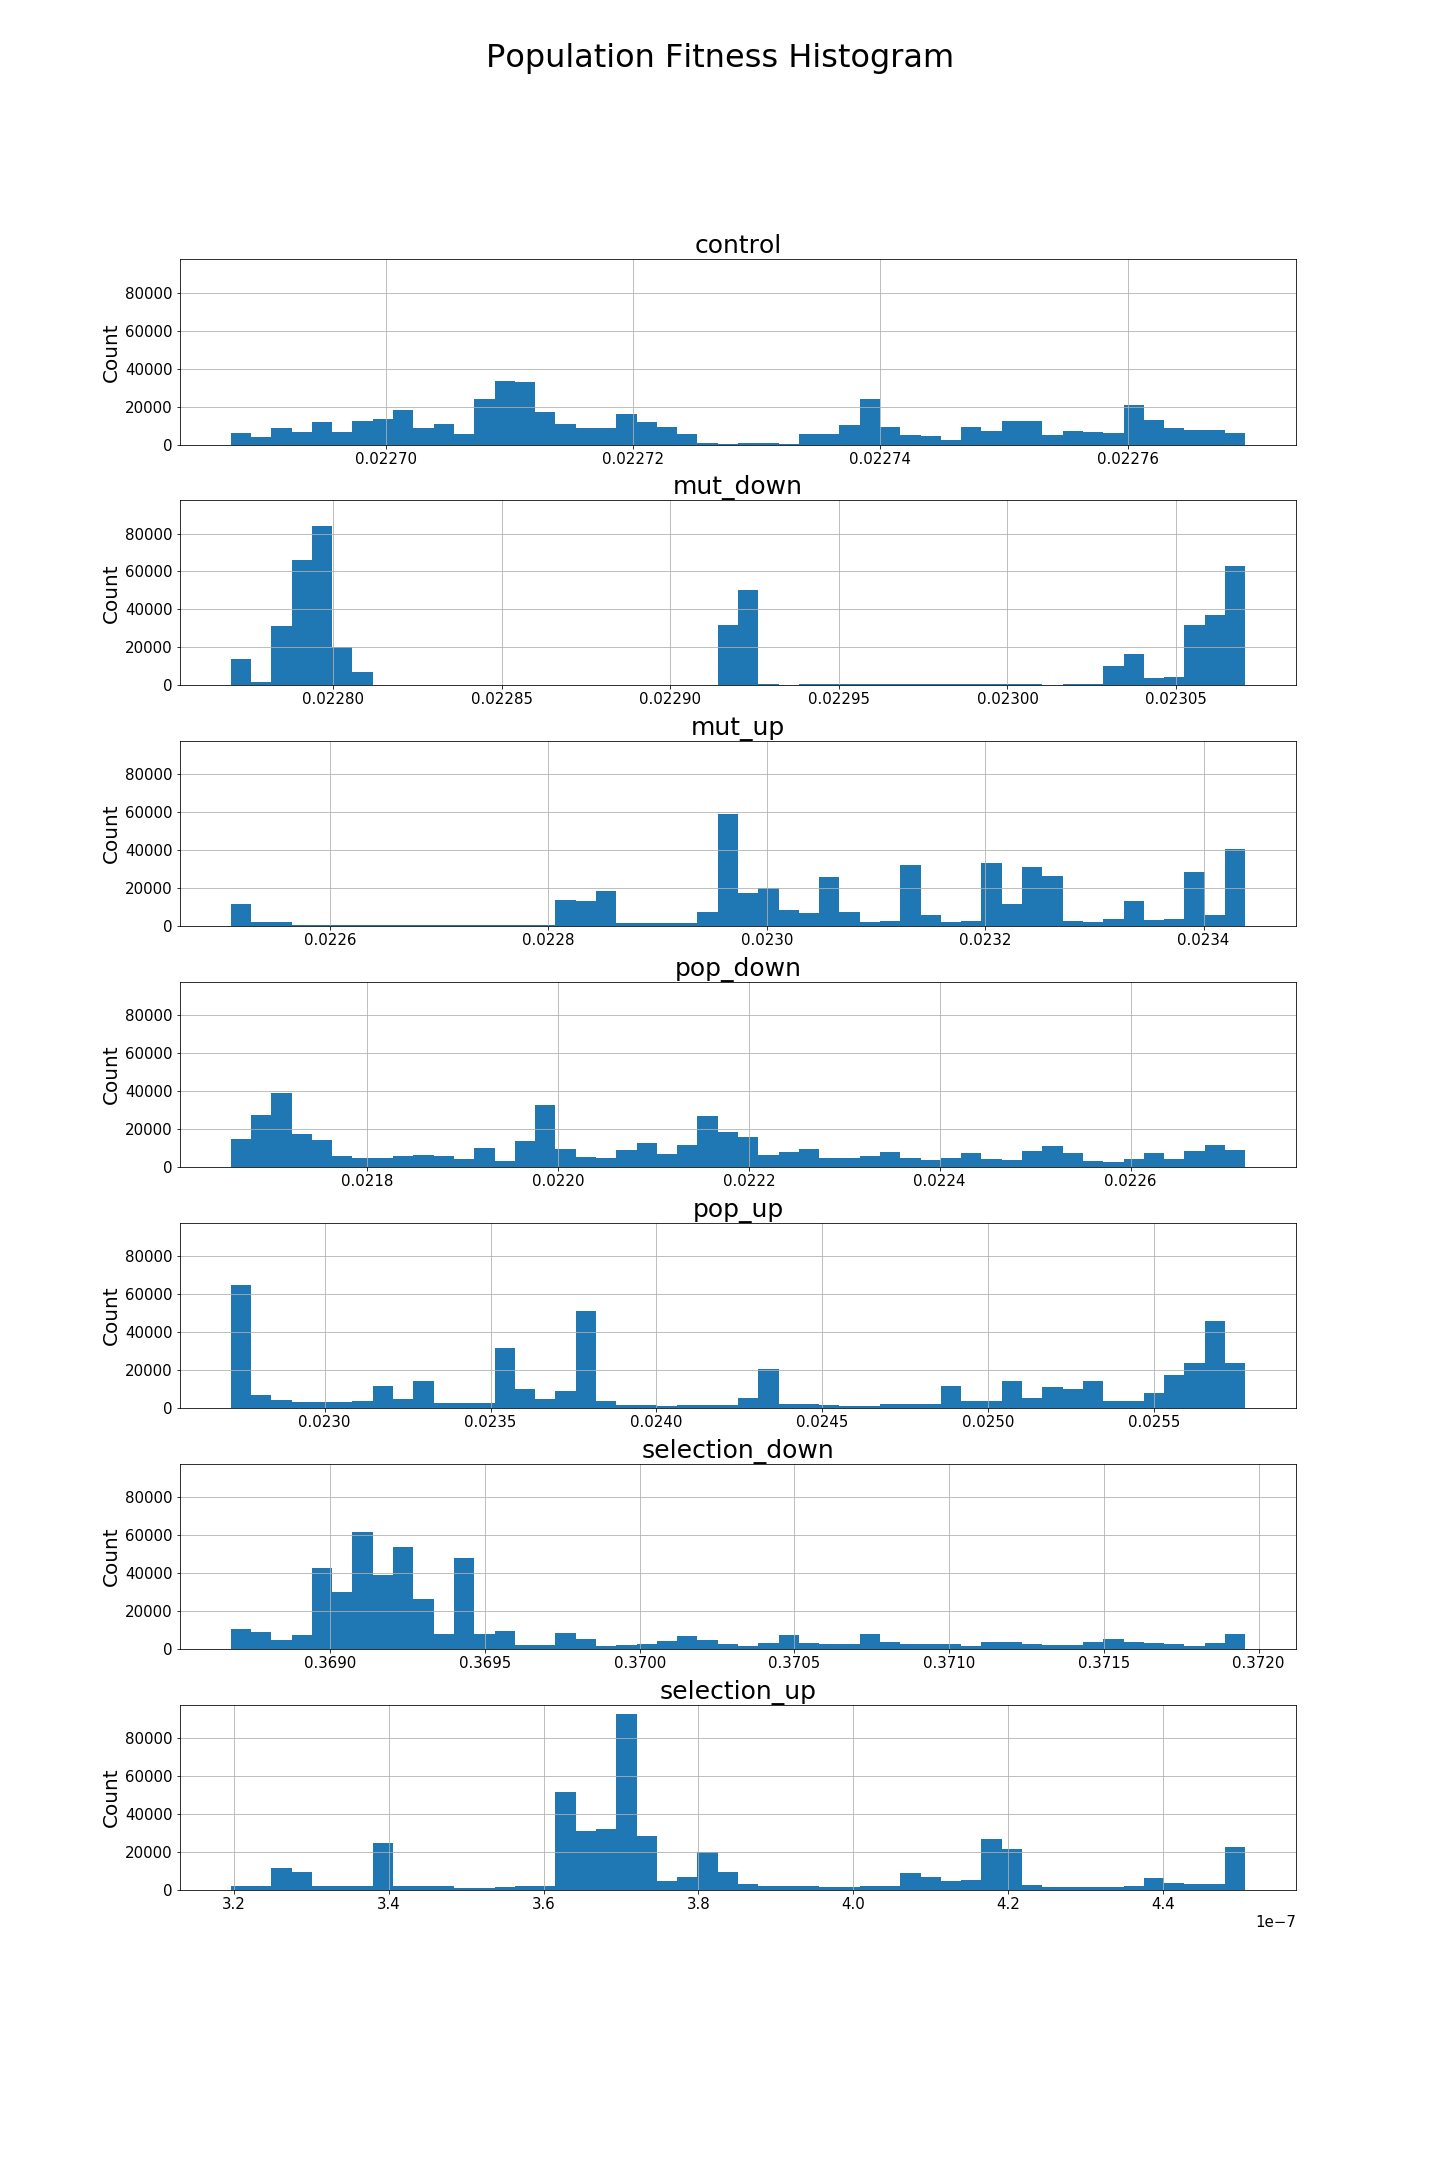
\includegraphics[width=\linewidth]{global_fitness_histogram}
	\caption[Mean fitness histogram]{Histogram of population fitness at generation 500,000 for all conditions. Note that for the selection up condition, the scale is 1e-7.}
	\label{fig:global_fitness_histogram}
\end{figure}
Figure~\ref{fig:global_fitness_histogram} shows a histogram of the population mean fitness values for all conditions over the 500k generations. Although the $N_-$ condition ended the simulations in the most similar position to the \textit{control} condition, Figure~\ref{fig:global_fitness_histogram} makes it clear that the \textit{control} condition remained much steadier throughout the simulation, regularly jumping from value to value, whereas the \textit{mutation down} condition, as expected, tended to hover at certain locations in between rarer mutation events. 

Figure~\ref{fig:mean_metabolic_error} shows the mean metabolic error across all seeds for the whole population over time with respect to each condition. 
\begin{figure}[H]
	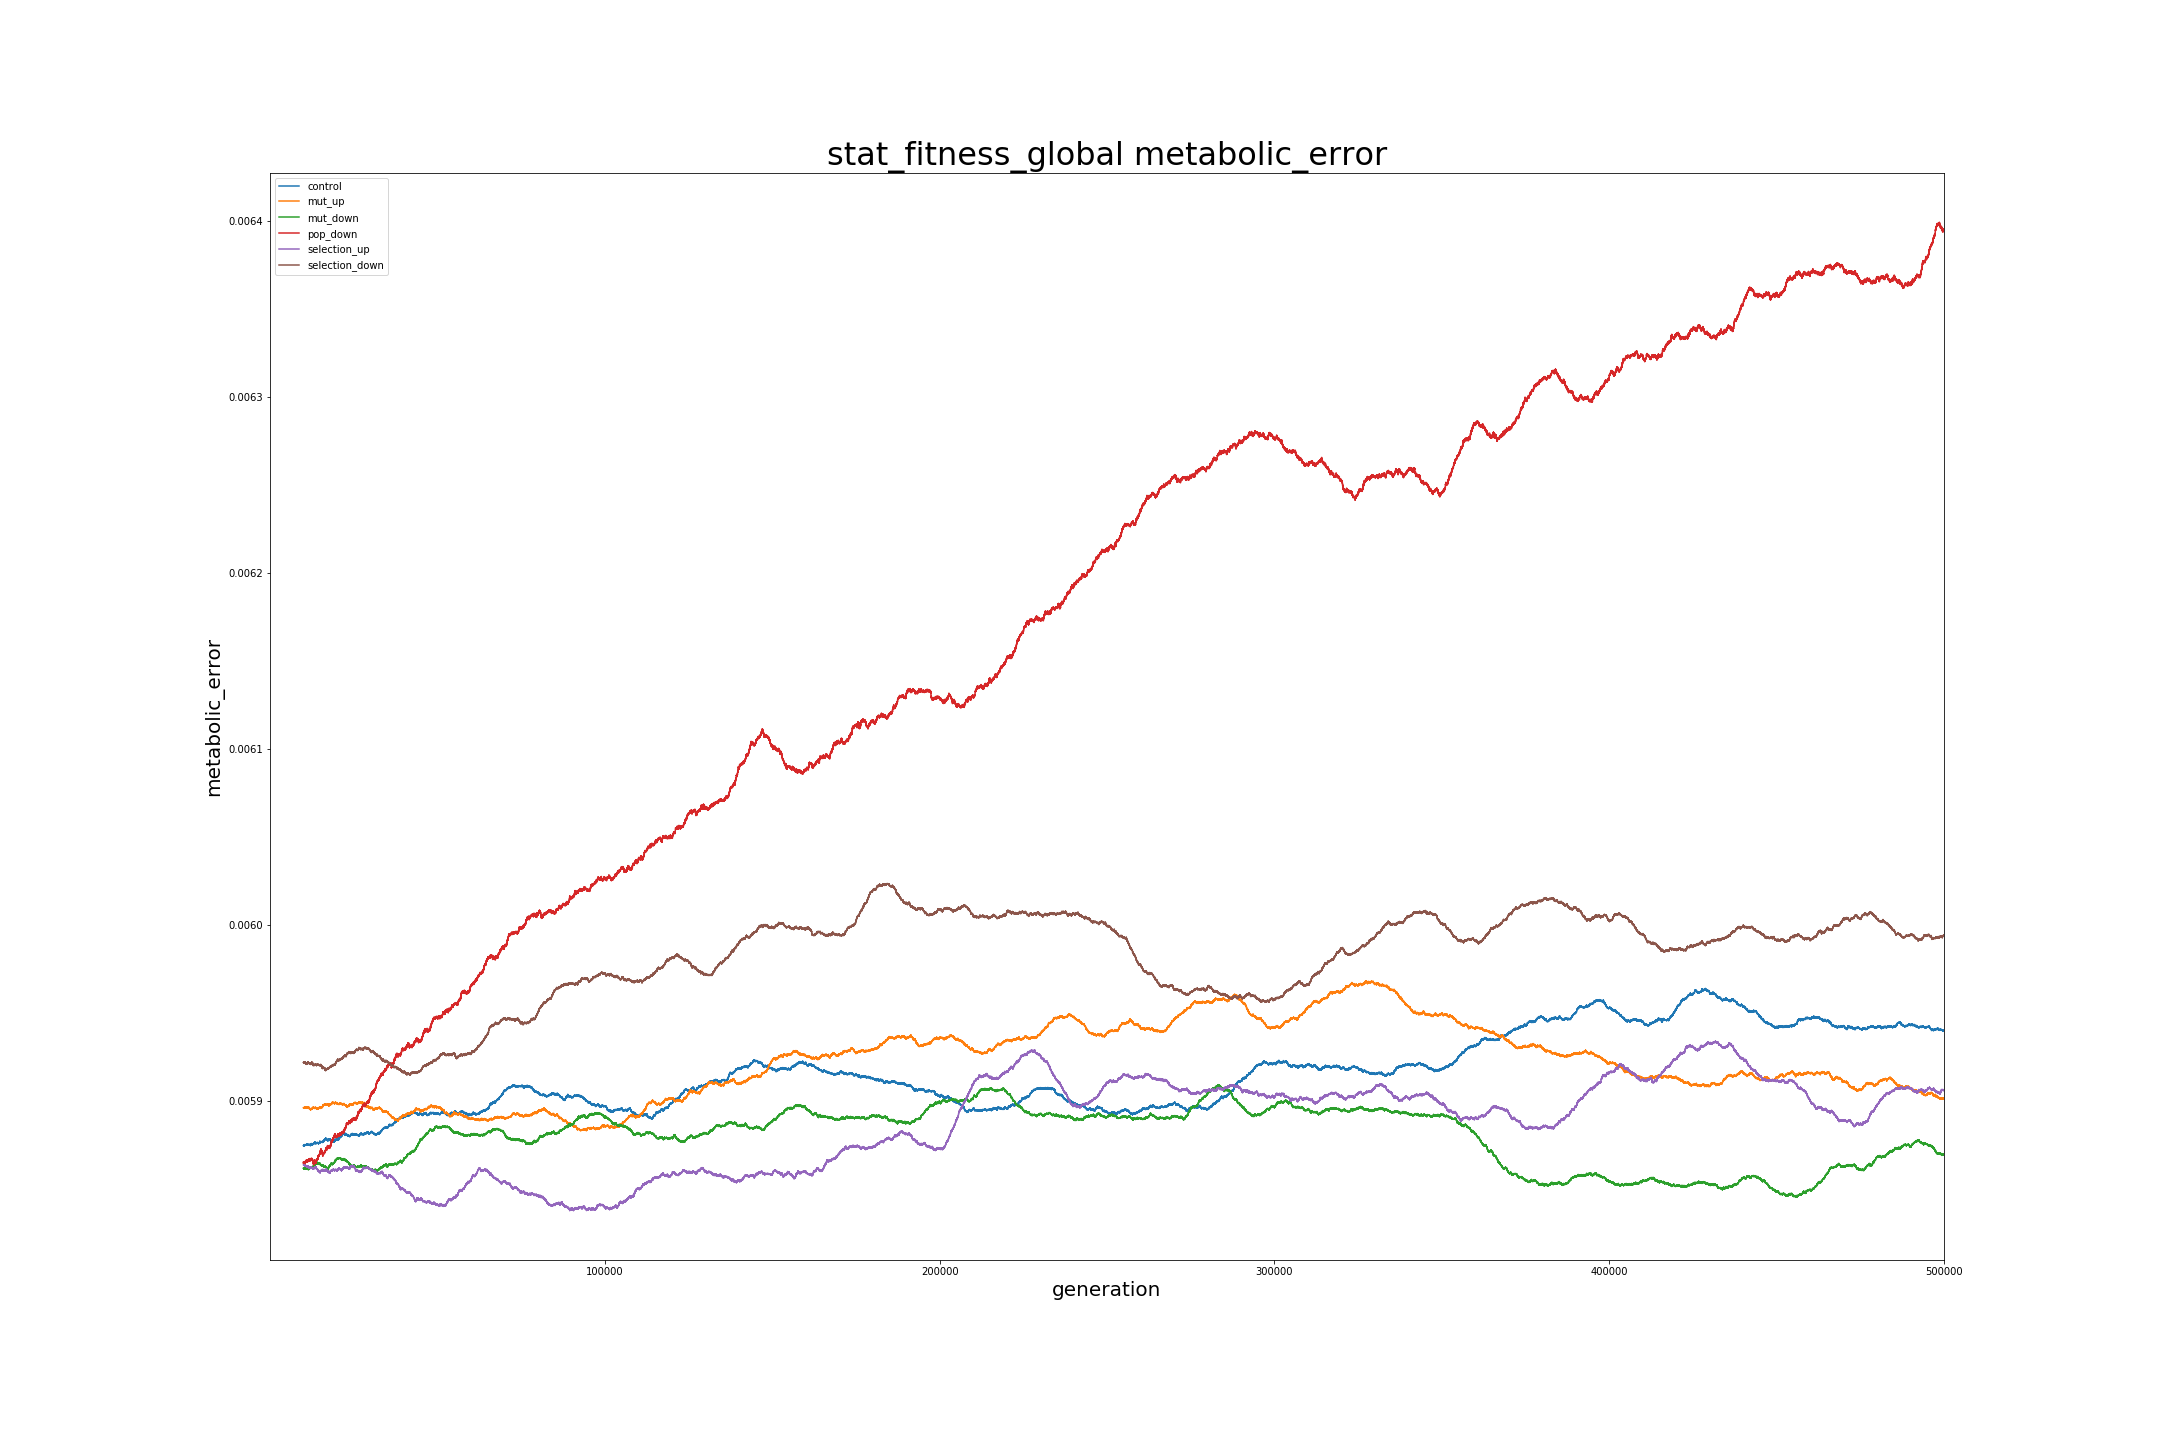
\includegraphics[width=\linewidth]{stat_fitness_global_mean_metabolic_error}
	\caption[Metabolic error]{Plot of the metabolic error over time for all conditions, average of all seeds}
	\label{fig:mean_metabolic_error}
\end{figure}

Table~\ref{table:fitness_means_std_dev} below gives the mean fitness scores for the population and the differing conditions. The selection down condition seems to be somewhat anomalous, as it was several orders of magnitude larger than all other conditions, despite having comparable genome sizes, numbers of genes, etc.
\begin{table}[H]
	\centering
	\begin{tabular}{|c||c|c|c|}
		\hline
		\multicolumn{4}{c}{\Large \textbf{Fitness}} \\
		\hline
		& \textbf{mean} & \textbf{standard deviation} & \textbf{mean's \% change from control} \\
		\hline \hline
		control & 2.272542e-02 & 2.34433e-05 & \textemdash \\ 
		\hline
		$\mu_+$ & 2.310701e-02 & 2.191826e-04 & 1.679131 \\ 
		\hline
		$\mu_-$ & 2.290879e-02 & 1.180940e-04 & 0.8068952 \\ 
		\hline
		$k_+$ & 3.803823e-07 & 3.130504e-08 & -99.99833 \\ 
		\hline
		$k_-$ & 3.695935e-01 & 8.101732e-04 & 1526.344 \\ 
		\hline
		$N_+$ & 2.428255e-02 & 1.081245e-03 & 6.851949 \\ 
		\hline
		$N_-$ & 2.209722e-02 & 3.104264e-04 & -2.764272 \\ 
		\hline
	\end{tabular}
	\caption[Fitness means and standard deviations.]{Population mean fitness, standard deviations, and percent change from the control condition across all seeds. }
	\label{table:fitness_means_std_dev}
\end{table}

\subsection{Genome Structure}
In this section, the effects of the differing conditions on the structure of the genome as measured by the criteria in Tables~\ref{table:aevol_stats_genes_and_bp} and~\ref{table:aevol_stats_fitness_and_mutation} is examined. 

\subsubsection{Non-coding DNA}
One important factor in genome structure is the amount of non-coding DNA, i.e. the number of bases which are part of a genome but which do not encode protein sequences. Aevol gives the number of bases which are not in any coding sequence, as well as the total genome size, so one may easily calculate this percentage. The results from the experiments are shown in Figure~\ref{fig:mean_non-coding_DNA}. Recalling genome size in Figure~\ref{fig:genome_size}, it seems that as the genome size of the population down condition rapidly expanded, most of those expansions were non-coding.
\begin{figure}[H]
	\centering
	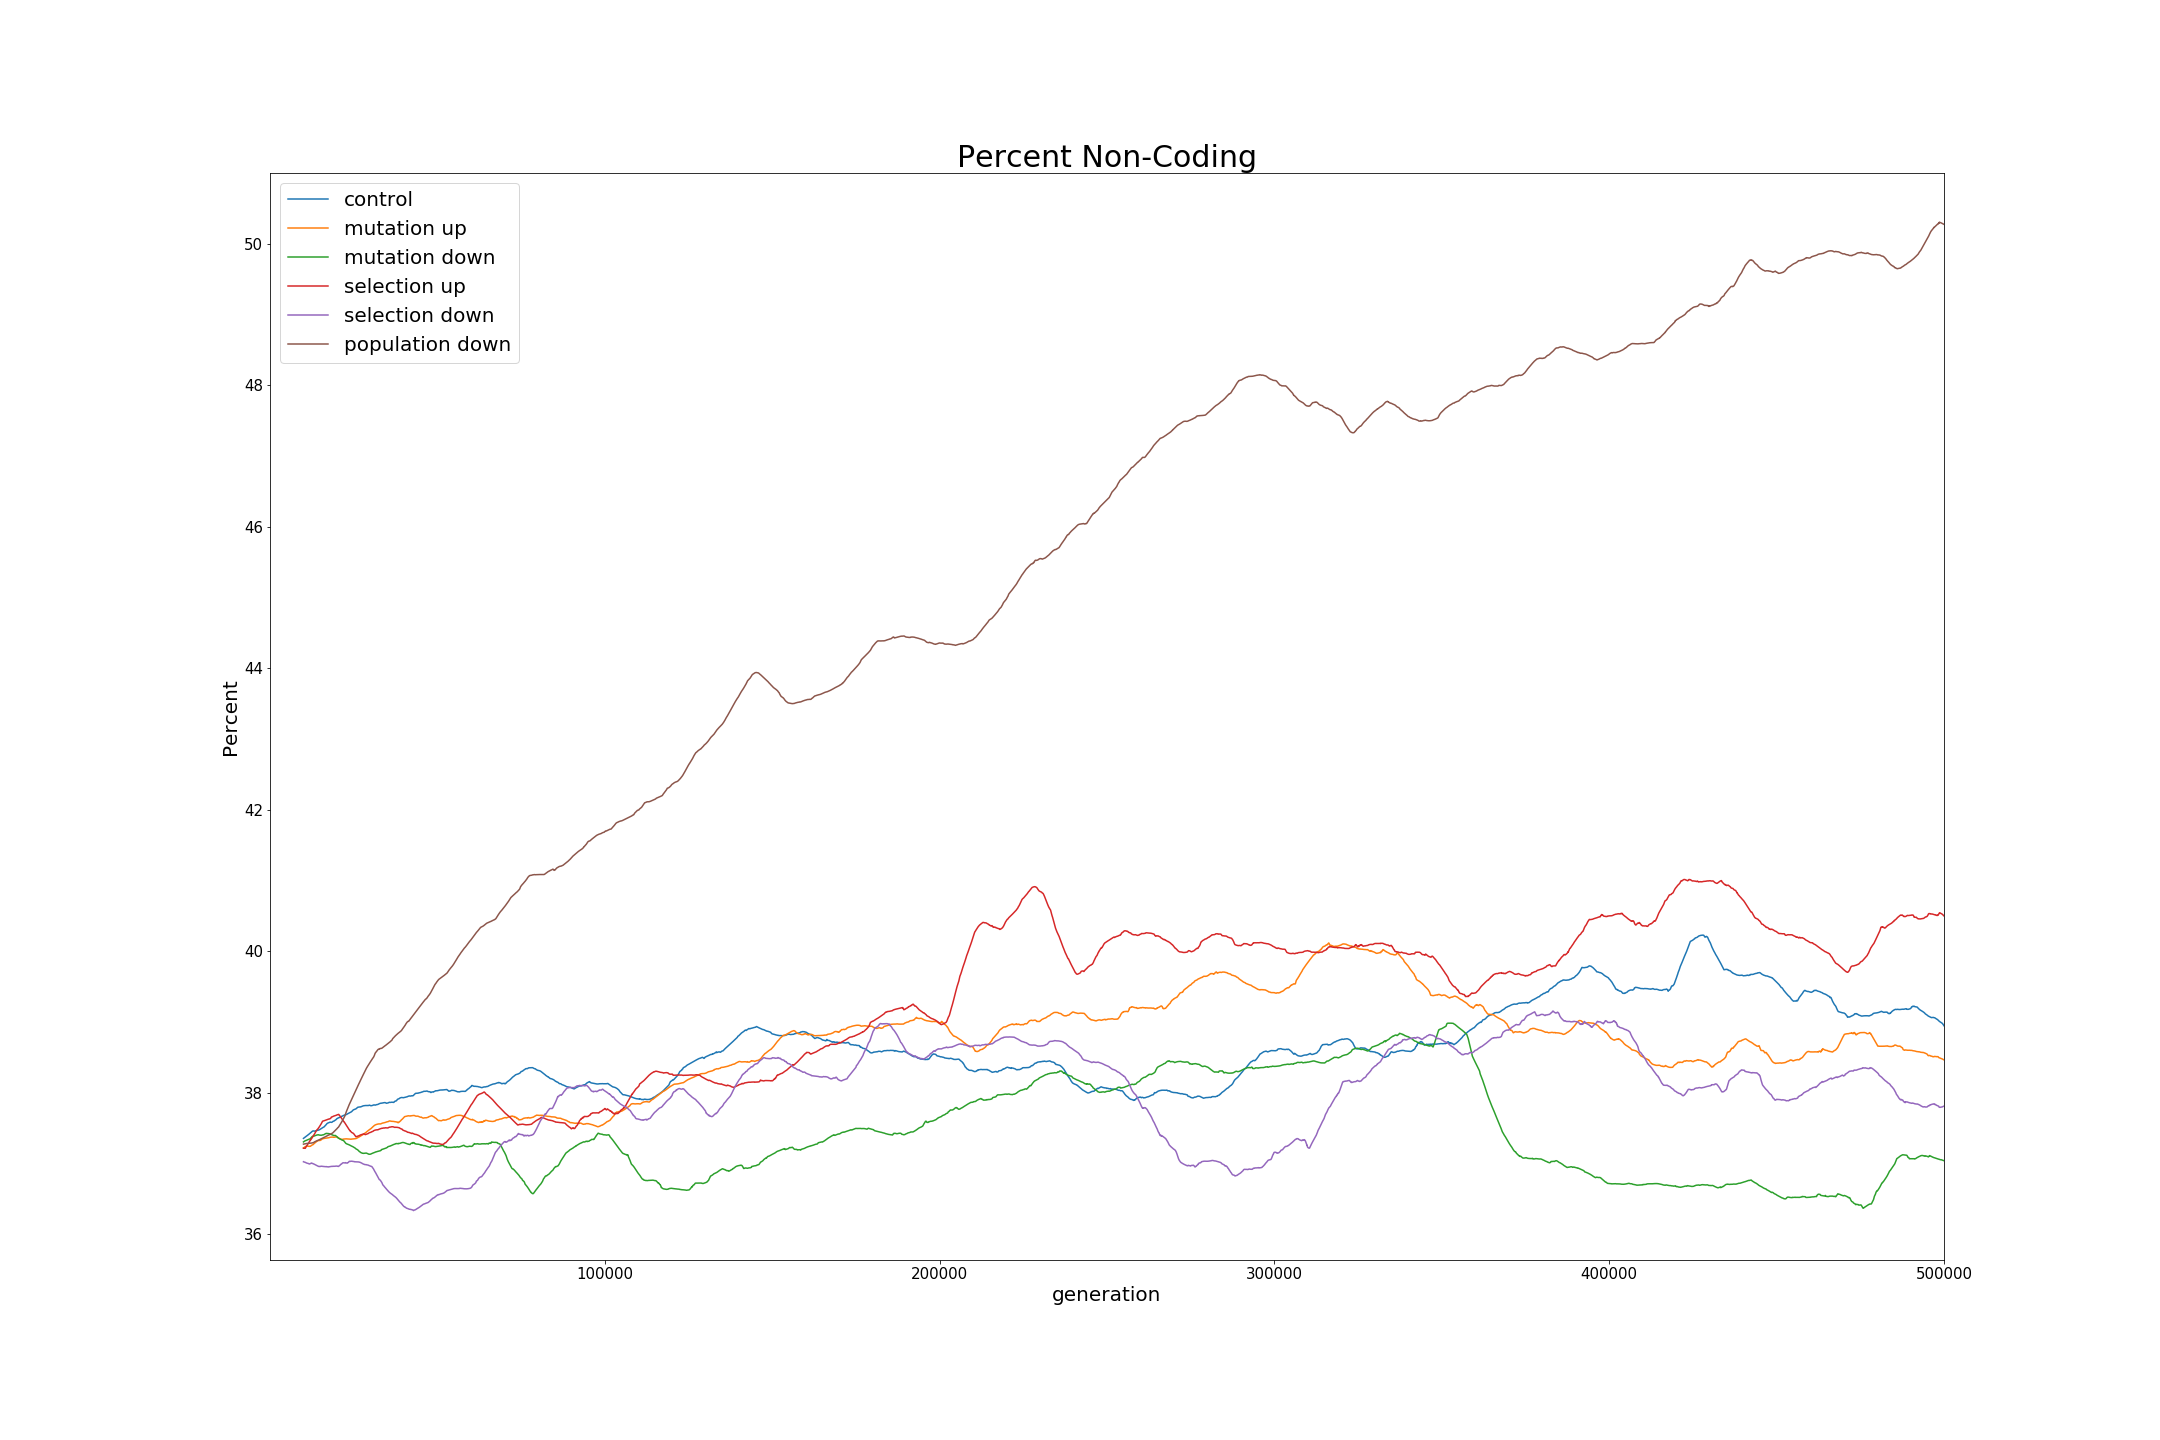
\includegraphics[width=\linewidth]{percent_noncoding}
	\caption[Non-coding DNA]{Plot of the average (across all seeds) number of non-coding bases for the whole population over time for all conditions.}
	\label{fig:mean_non-coding_DNA}
\end{figure}
By comparison, despite the $k_+$ condition's rapid decline in fitness, it did not acquire more than 1\% non-coding DNA. 

The average percentages of non-coding DNA are given in Table~\ref{table:non-coding_DNA_mean_and_standard_deviation} below. 
\begin{table}[H]
	\begin{tabular}{|c|c|c|c|}
		\hline
		\multicolumn{4}{c}{\Large \textbf{\% Non-coding DNA}} \\
		\hline
		& \textbf{mean} & \textbf{standard deviation} & \textbf{mean's \% change from control} \\
		\hline \hline
		control & 38.622711 & 0.601258 & \textemdash \\ 
		\hline
		$\mu_+$ & 38.661764 & 0.707173 & 0.101114 \\ 
		\hline
		$\mu_-$ & 37.446414 & 0.694349 & -3.045608 \\ 
		\hline
		$k_+$ & 39.329164 & 1.138623 & 1.829114 \\ 
		\hline
		$k_-$ & 38.004029 & 0.704953 & -1.601860 \\ 
		\hline
		$N_-$ & 45.462209 & 3.545778 & 17.708489 \\ 
		\hline
	\end{tabular}
	\caption[Non-coding DNA mean and standard deviation]{Mean and standard deviation of non-coding percentages of DNA across all seeds.}
	\label{table:non-coding_DNA_mean_and_standard_deviation}
\end{table}

\subsubsection{Number of Functional Genes}\label{sec:number_of_functional_genes}
Recall from Section~\ref{experimental_design} that a ``functional gene'' is a gene which produces a gene product. Specifically in Aevol, this means the production of a triangle of mean $m$, height $h$, and half-width $w$. Figure~\ref{fig:mean_num_functional_genes} below illustrates the mean number of functional genes across the population for each condition.  
\begin{figure}[H]
	\centering
	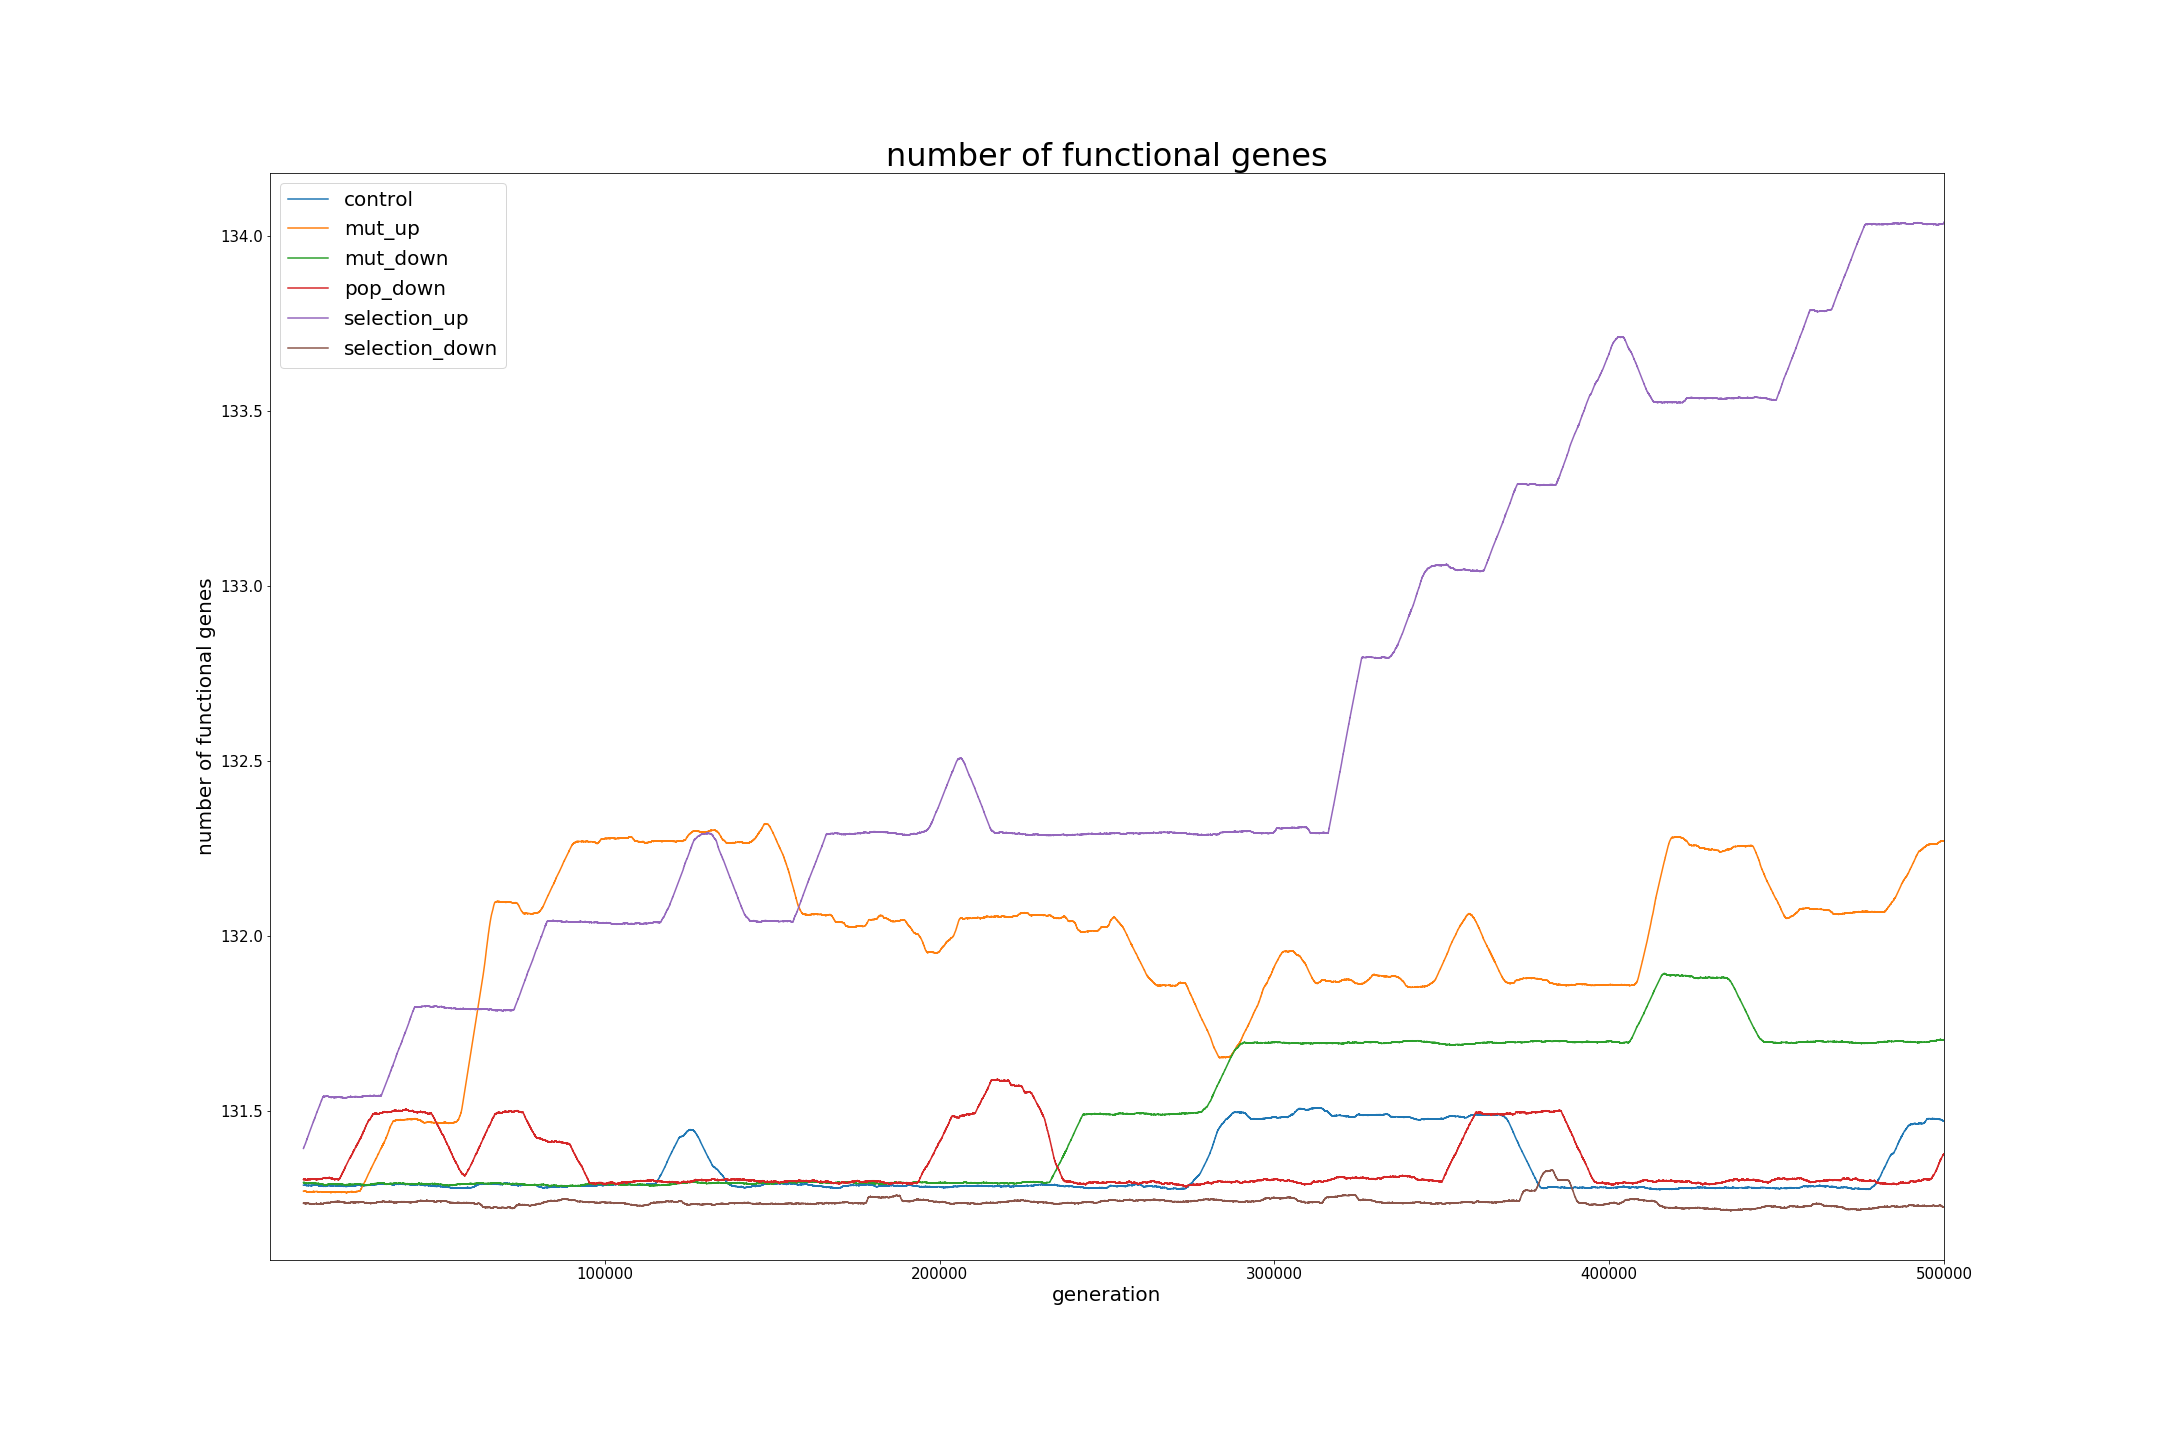
\includegraphics[width=\linewidth]{stat_genes_global_mean_num_functional_genes}
	\caption[Mean number of functional genes]{Plot showing the mean number of functional genes for the population, averaged across all seeds for each condition.}
	\label{fig:mean_num_functional_genes}
\end{figure}
As seen in the figure, the \textit{selection up} condition showed the greatest increase in the number of functional genes in the whole population, reaching a maximum increase of about 2.2\% (131 to 134). This is in agreement with the predictions (from Table~\ref{table:experiment_predictions}) and the findings of Knibbe et al.~\cite{Knibbe2007}. Whereas most of the other curves are fairly flat, the mutation up condition fluctuates relatively rapidly, owing to the quick increase and decrease in the number of base pairs. 

The mean and standard deviation of the number of functional genes for the population for each condition is given in Table~\ref{table:number_of_genes_mean_std_dev} below.

\begin{table}[H]
	\centering
	\begin{tabular}{|c|c|c|c|}
		\hline
		\multicolumn{4}{c}{\Large \textbf{Mean Number of Functional Genes}} \\
		\hline
		& \textbf{mean} & \textbf{standard deviation} & \textbf{\% change from control} \\
		\hline
		control & 131.332898 & 0.081508 & \textemdash \\ 
		\hline
		$\mu_+$ & 131.974778 & 0.252463 & 0.488742 \\ 
		\hline
		$\mu_-$ & 131.500541 & 0.207570 & 0.127647 \\ 
		\hline
		$k_+$ & 132.606568 & 0.719530 & 0.969803 \\ 
		\hline
		$k_-$ & 131.238909 & 0.013974 & -0.071565 \\ 
		\hline
		$N_-$ & 131.350519 & 0.083280 & 0.013417 \\ 
		\hline
	\end{tabular}
	\caption[Number of functional genes - mean and standard deviation]{The mean and standard deviation for the number of functional genes of the population, averaged across all seeds and for all conditions.}
	\label{table:number_of_genes_mean_std_dev}
\end{table}
\subsubsection{Number of Non-Functional Genes}
The average number of non-functional genes across all seeds for each condition is illustrated in Figure~\ref{fig:mean_num_non-functional_genes} below, and Table~\ref{table:non-functional_genes_mean_std_dev} provides the mean and standard deviation for all seeds and all conditions.  

\begin{figure}[H]
	\centering
	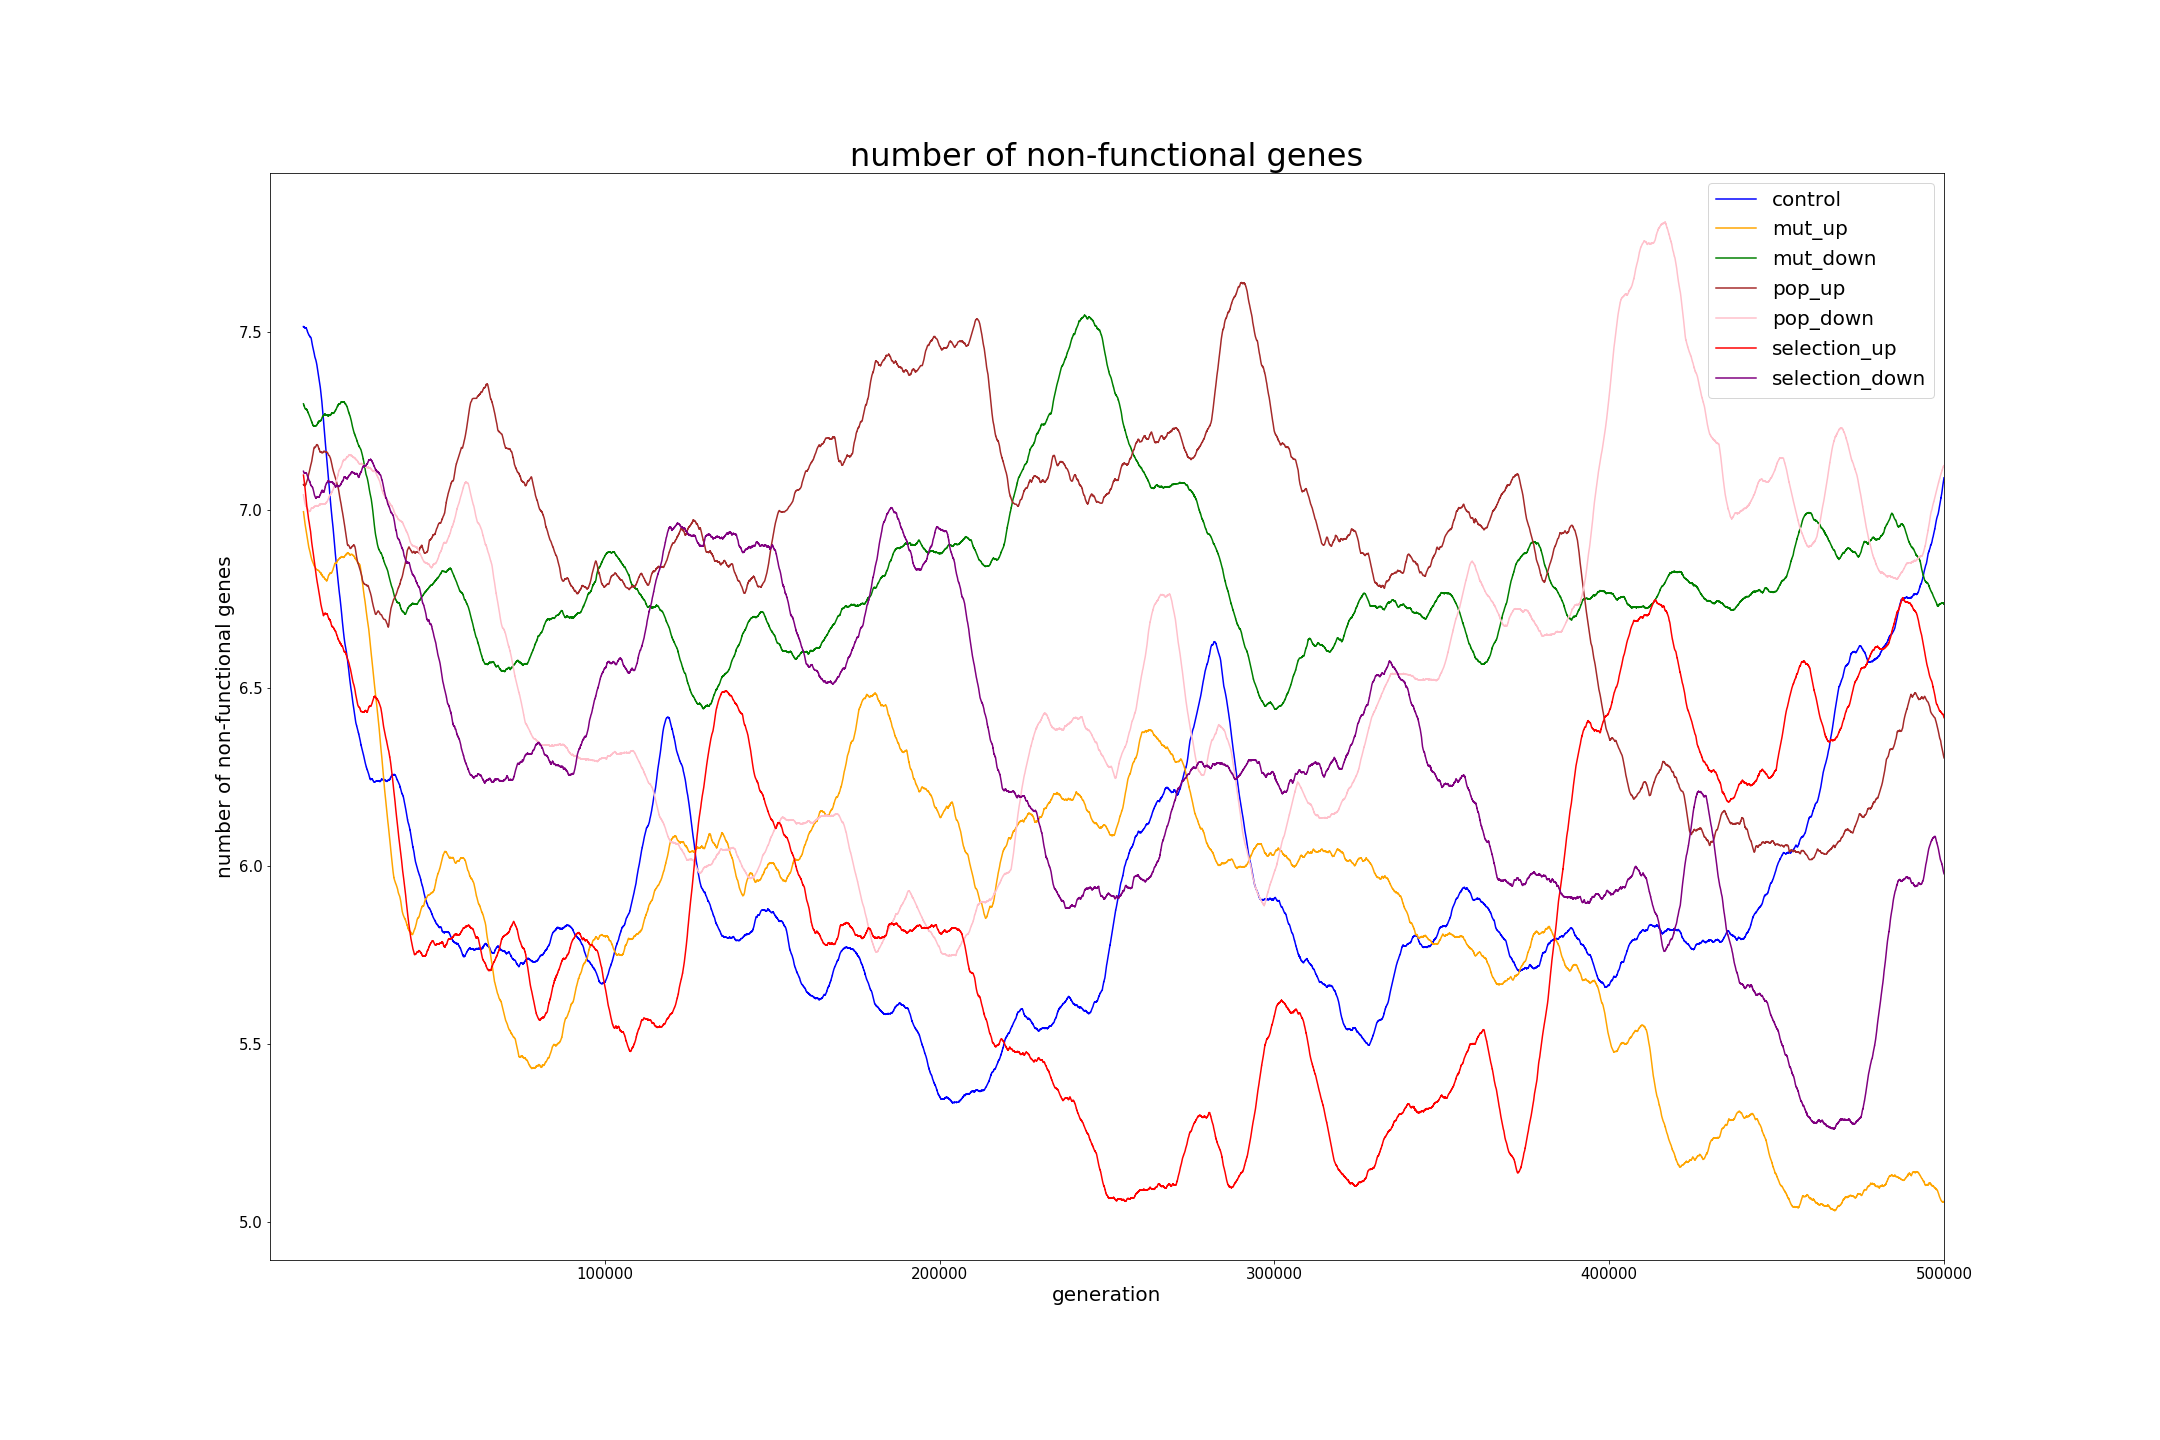
\includegraphics[width=\linewidth]{stat_genes_global_mean_num_non-functional_genes}
	\caption[Mean number of non-functional genes]{The mean number of non-functional genes across all seeds for each condition.}
	\label{fig:mean_num_non-functional_genes}
\end{figure}


\begin{table}[h]
	\centering
	\begin{tabular}{|c|c|c|c|}
		\hline
		\multicolumn{4}{c}{\Large \textbf{Population Mean Number of Non-Functional Genes - Mean \& Std. Dev.}} \\
		\hline
		& \textbf{mean} & \textbf{standard deviation} & \textbf{\% change from control} \\
		\hline
		control & 5.927067 & 0.385790 & \textemdash \\ 
		\hline
		$\mu_+$ & 5.856449 & 0.428473 & -1.191458 \\ 
		\hline
		$\mu_-$ & 6.821348 & 0.221591 & 15.088075 \\ 
		\hline
		$k_+$ & 5.844289 & 0.506922 & -1.396610 \\ 
		\hline
		$k_-$ & 6.297804 & 0.454152 & 6.254978 \\ 
		\hline
		$N_-$ & 6.555471 & 0.483631 & 10.602267 \\ 
		\hline
	\end{tabular}
	\caption[Number of Non-functional Genes - Mean \& St. Dev.]{Population mean and standard deviation for the number of non-functional genes, mean of all seeds, all conditions.}
	\label{table:non-functional_genes_mean_std_dev}
\end{table}

\subsubsection{Average Size of Functional Genes}\label{sec:average_size_functional_genes}
Figure~\ref{fig:mean_functional_gene_size} shows the average number of base pairs for each functional gene for the population, mapped out over the 500,000 generations. The population down condition continues to be the outlier in terms of genome structure, with the average size of the functional genes remaining noticeably lower than for any other condition. It is worth pointing out, however, that the difference between the smallest average and the largest average is only 1 base pair. 
\begin{figure}[H]
	\centering
	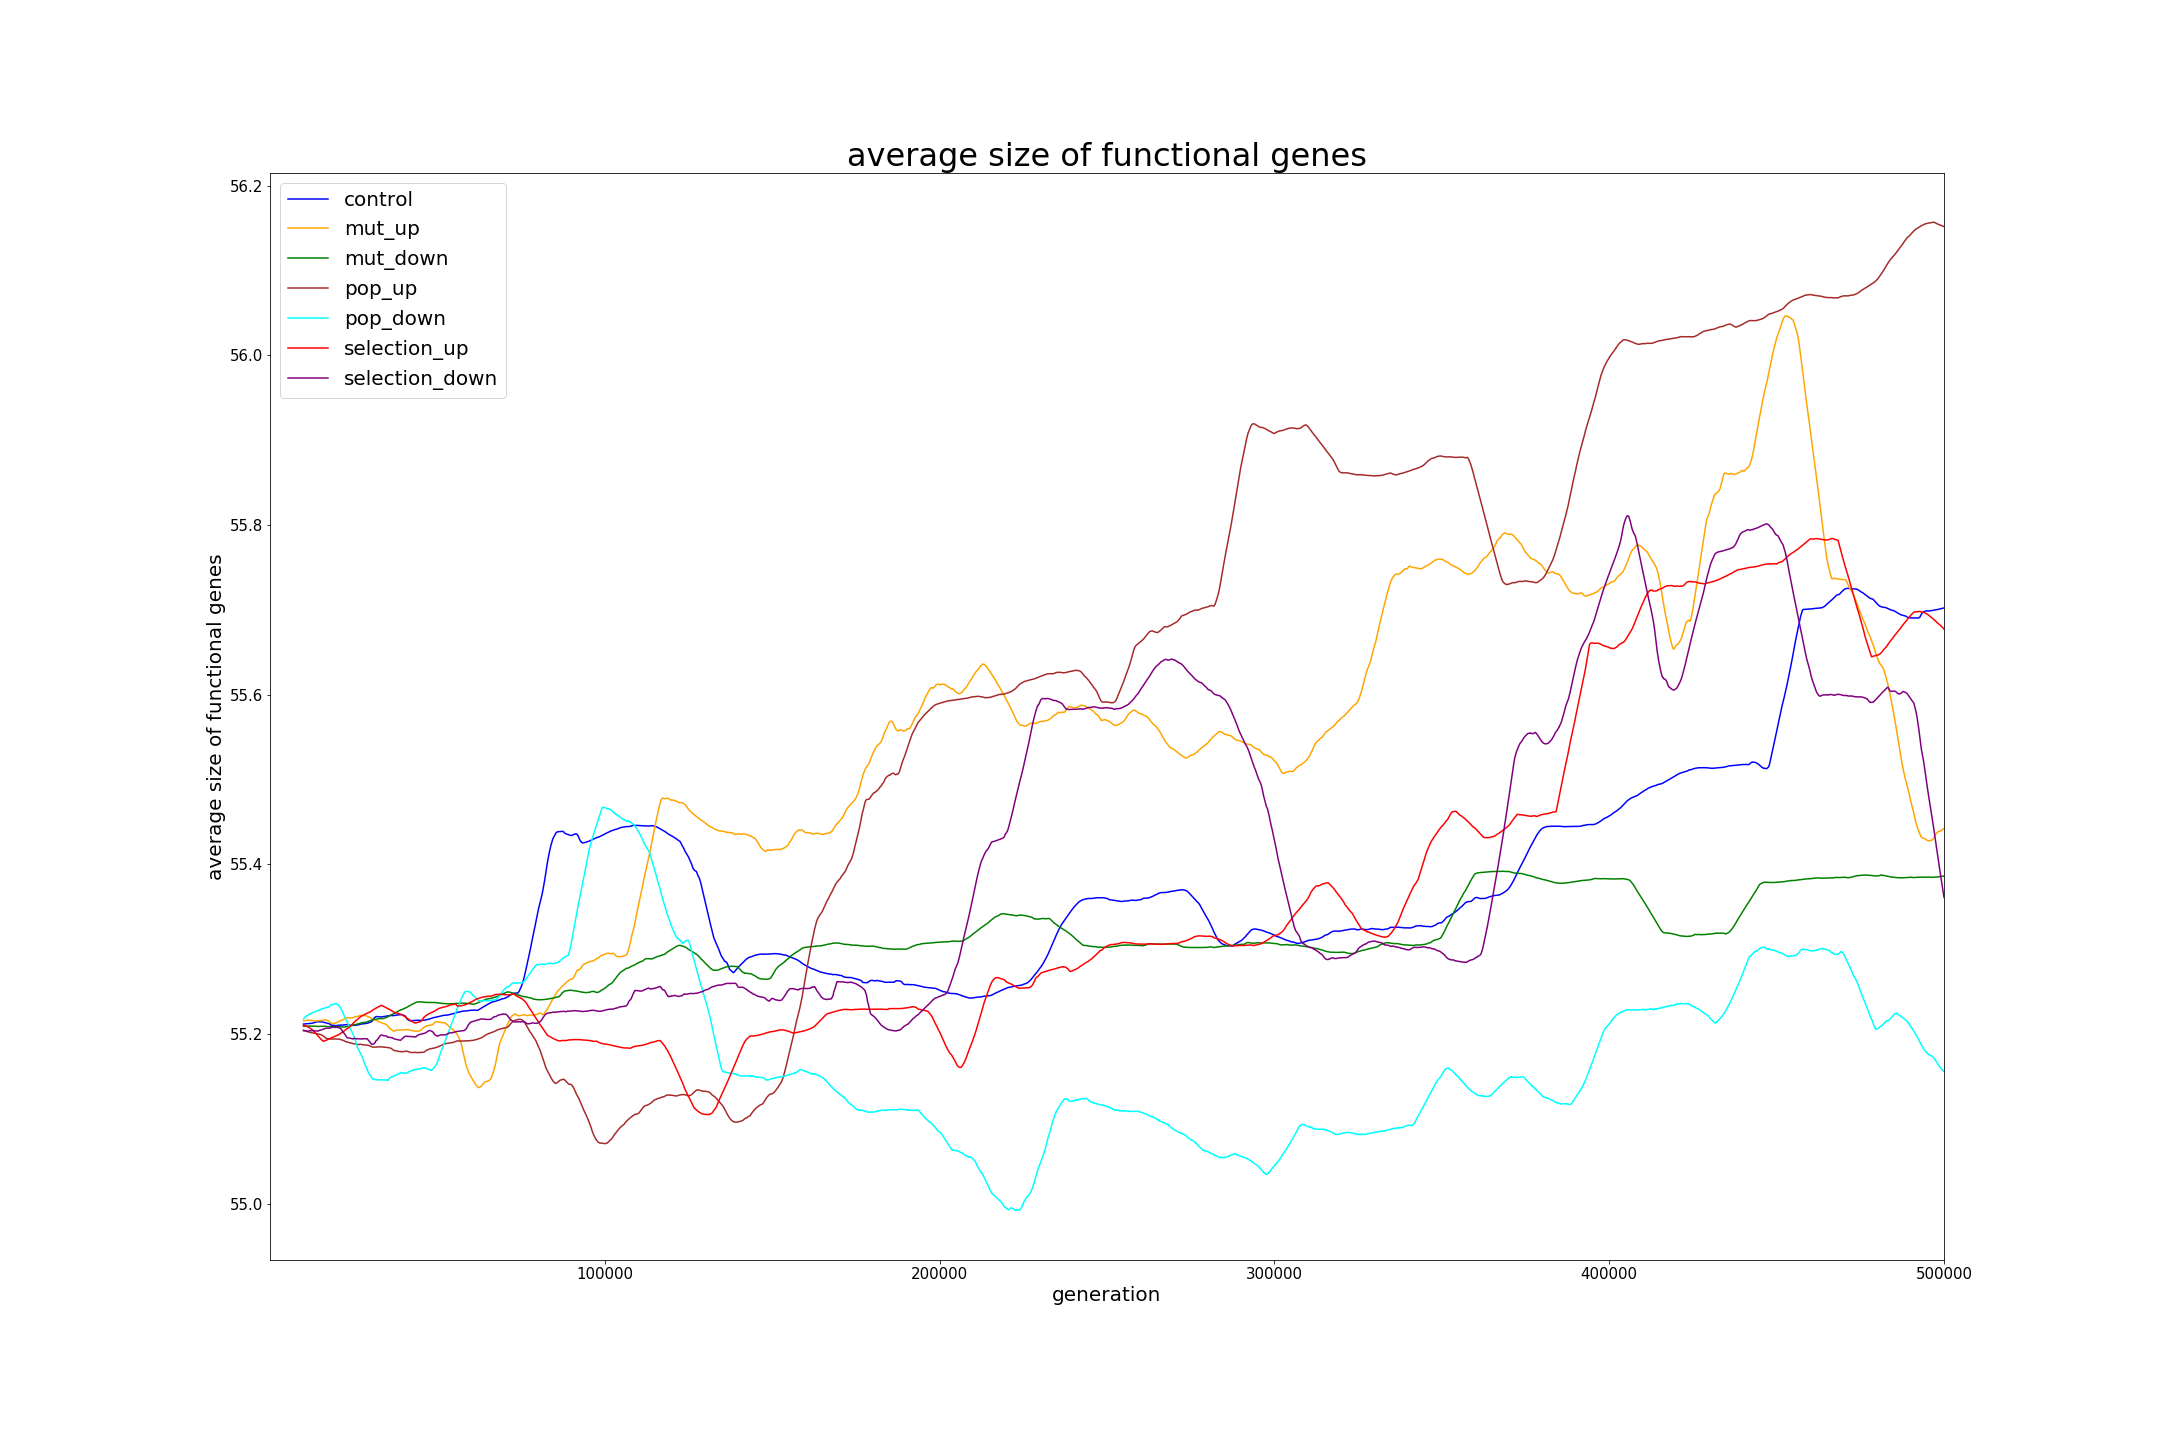
\includegraphics[width=\linewidth]{stat_genes_global_mean_avg_size_of_functional_genes}
	\caption[Average size of functional genes]{Plot showing the average size of functional genes over time for all seeds.}
	\label{fig:mean_functional_gene_size}
\end{figure}
Table~\ref{table:mean_functional_gene_size_and_std_dev} below gives the mean and standard deviation of the results, and Table~\ref{table:avg_size_of_functional_genes_rank_sum_and_p-value} gives the p-values for comparing the control condition to every other condition. 

\begin{table}[H]
	\centering
	\begin{tabular}{|c|c|c|c|}
		\hline
		\multicolumn{4}{c}{\Large \textbf{Average size of functional genes}} \\
		\hline
		& \textbf{mean} & \textbf{standard deviation} & \textbf{\% change from control} \\
		\hline
		control & 55.375430 & 0.137457 & \textemdash \\ 
		\hline
		$\mu_+$ & 55.542625 & 0.207164 & 0.301929 \\ 
		\hline
		$\mu_-$ & 55.309915 & 0.050594 & -0.118309 \\ 
		\hline
		$k_+$ & 55.370465 & 0.202443 & -0.008965 \\ 
		\hline
		$k_-$ & 55.414465 & 0.195425 & 0.070492 \\ 
		\hline
		$N_-$ & 55.174290 & 0.098860 & -0.363230 \\ 
		\hline
	\end{tabular}
	\caption[Mean functional gene size and standard deviation]{Mean functional gene size and standard deviation, all seeds, all conditions.}
	\label{table:mean_functional_gene_size_and_std_dev}
\end{table}

\begin{table}[H]
	\begin{tabular}{|c|c|c|}
		\hline
		\multicolumn{3}{c}{\Large \textbf{Average size of functional genes - rank sum \& p-value}} \\
		\hline
		& \textbf{rank sum} & \textbf{p-value} \\
		\hline
		$\mu_+$ & 68252491056.00 & 0.00000000 \\ 
		\hline
		$\mu_-$ & 96067062201.50 & 0.00000000 \\ 
		\hline
		$N_-$ & 28963878467.00 & 0.00000000 \\ 
		\hline
		$k_+$ & 103481641646.00 & 0.00000000 \\ 
		\hline
		$k_-$ & 124890321462.00 & 0.22366471 \\ 
		\hline
	\end{tabular}
	\caption[Average size of functional genes - rank sum and p-value]{Average size of functional genes - rank sum and p-value for all conditions and all seeds.}
	\label{table:avg_size_of_functional_genes_rank_sum_and_p-value}
\end{table}
Since the $k_-$ condition's p-value was $\geq0.05$, it must be concluded that these results are not significant. 

\subsection{Evolvability}
In Figure~\ref{fig:evolvability_mean} below, the results of the experiments on evolvability for the best individual's (at generation 500,000) lineage are shown. 
\begin{figure}[H]
	\centering
	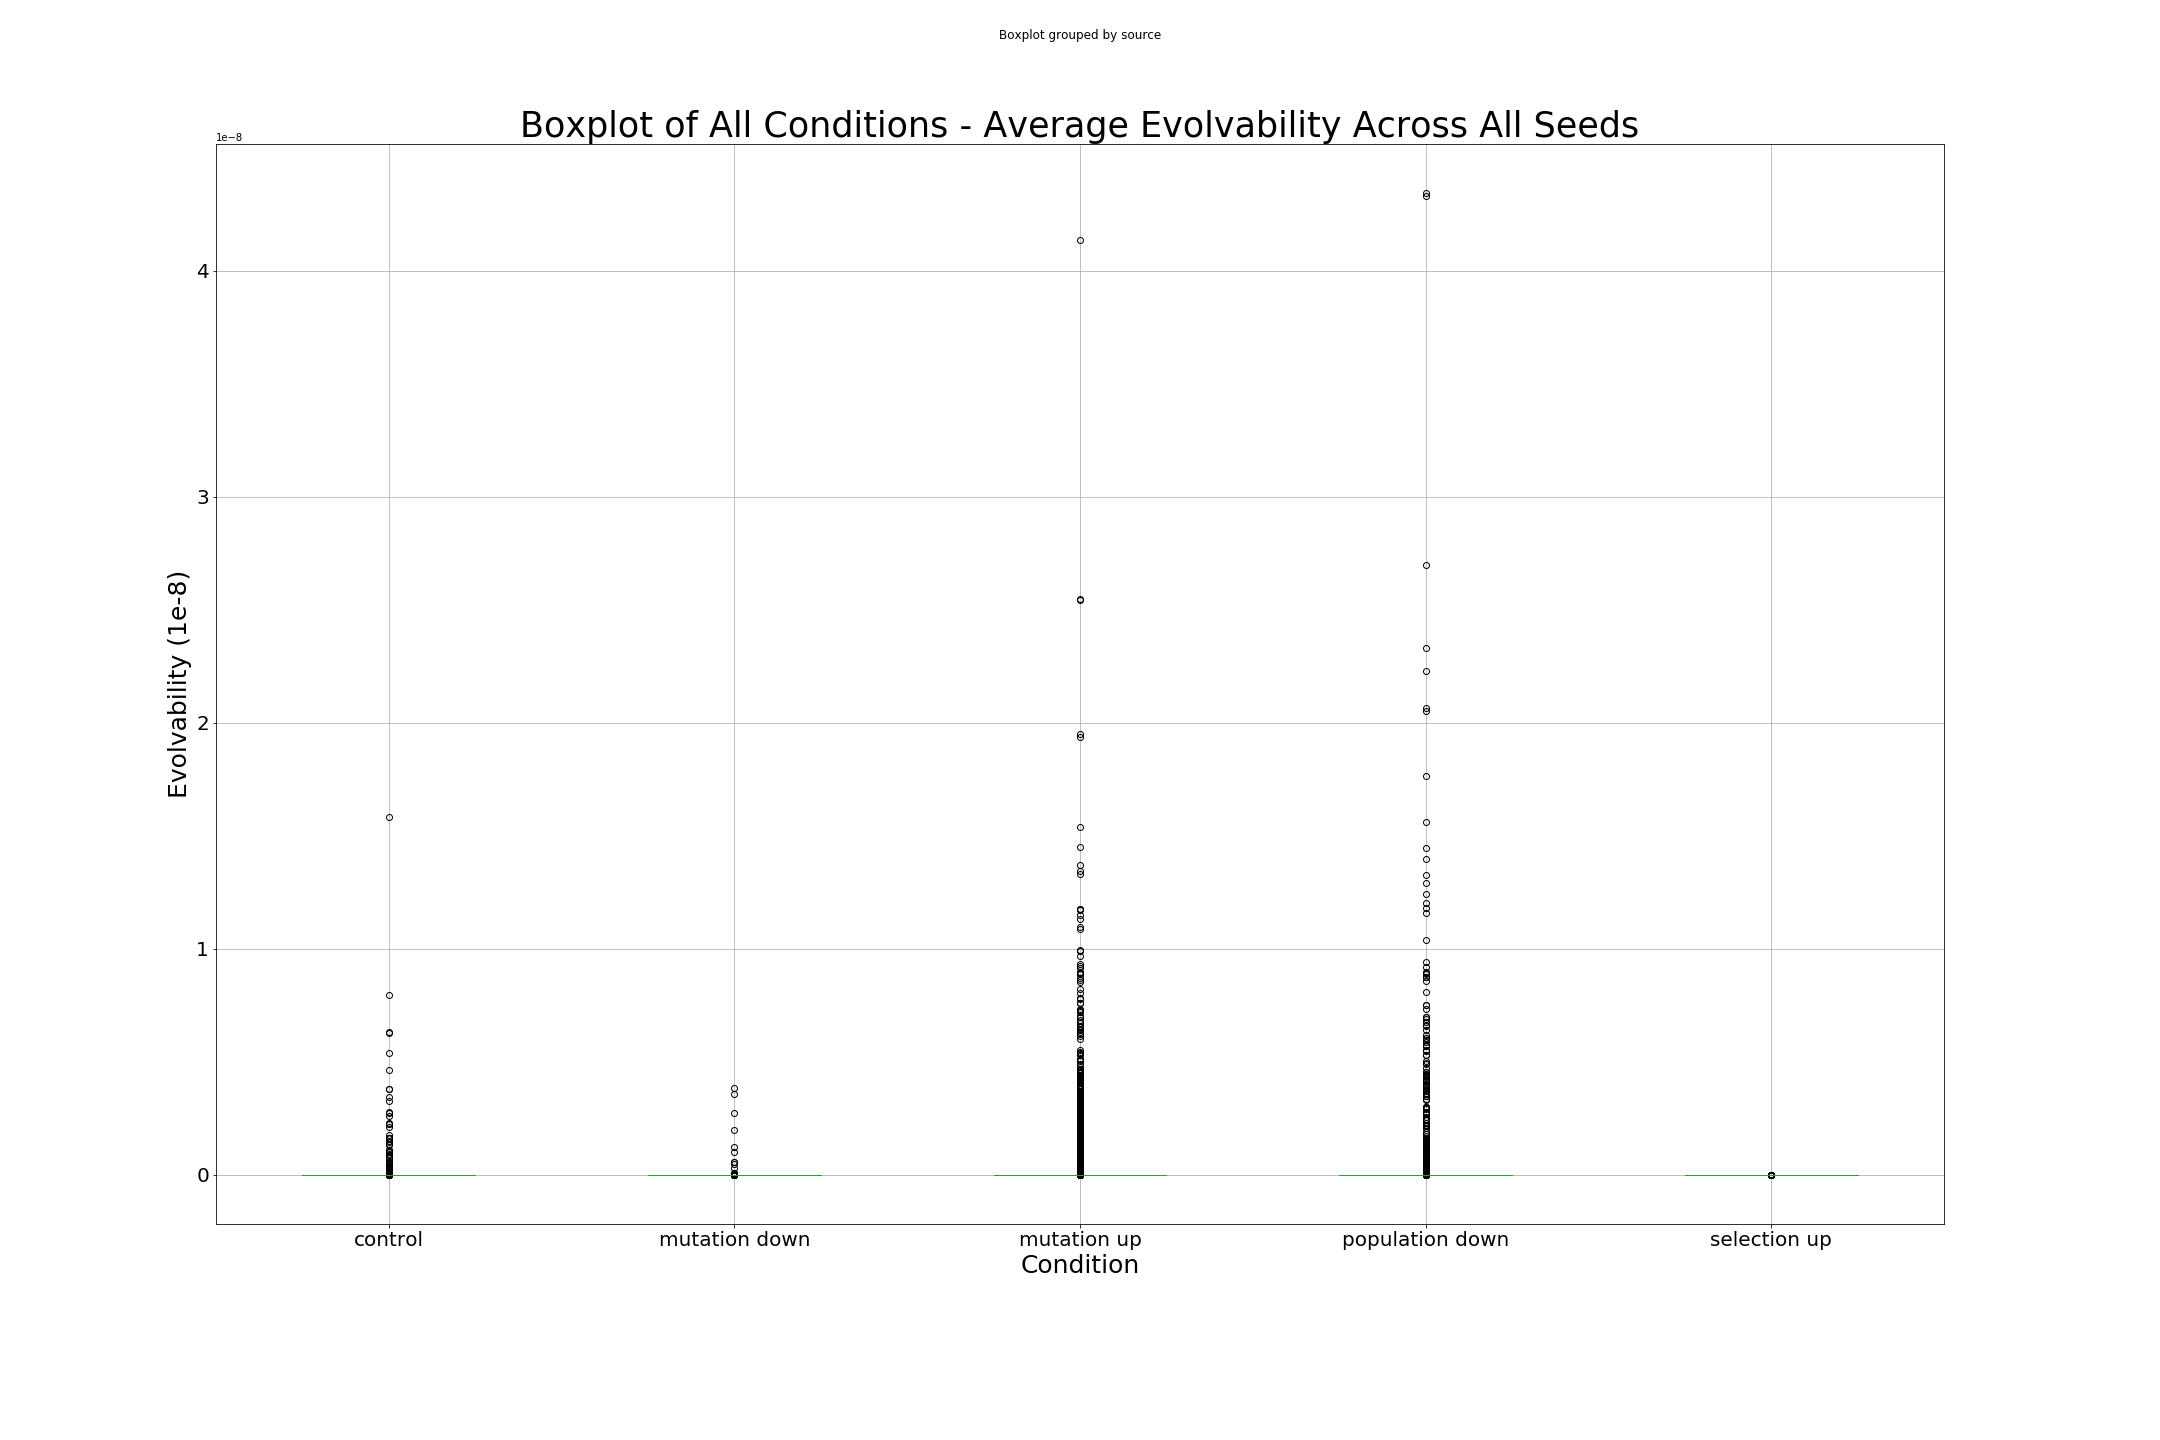
\includegraphics[width=\linewidth]{evolvability_boxplot_all_seeds_avg}
	\caption[Evolvability boxplot]{A box and whisker plot showing the mean evolvability spread of all seeds and all conditions. Larger numbers are more evolvable (keep in mind the scale is $1e^{-8}$). }
	\label{fig:evolvability_mean}	
\end{figure}
The figure illustrates that, for each condition, overall the best individual still had quite low evolvability. For the selection up condition, however, the deviation from zero was even smaller, as illustrated in Table~\ref{table:mean_std_dev_evolvability} below, which provides the mean and standard deviation of the evolvability of the best individual in each condition. 

The evolvability rank sum and p-value information is given in Table~\ref{table:evolvability-rank_sum_and_p-values}.

\begin{table}[H]
	\begin{tabular}{|c|c|c|}
		\hline
		\multicolumn{3}{c}{\Large \textbf{Evolvability rank sum and p-value}} \\
		\hline
		& \textbf{rank sum} & \textbf{p-value} \\
		\hline
		$\mu_+$ & 36203620.00 & 0.00000000 \\ 
		\hline
		$\mu_-$ & 7025283.50 & 0.01021245 \\ 
		\hline
		$N_-$ & 19403134.50 & 0.00000000 \\ 
		\hline
		$k_+$ & 13181851.50 & 0.00000000 \\ 
		\hline
		$k_-$ & 13779001.50 & 0.00000008 \\ 
		\hline
	\end{tabular}
	\caption[Evolvability - rank sum and p-value]{Rank sum and p-values for evolvability, all seeds, all conditions.}
	\label{table:evolvability-rank_sum_and_p-values}
\end{table}

\begin{table}[H]
	\centering
	\begin{tabular}{| c | c | c | c |}
		\hline
		\multicolumn{4}{c}{\Large Evolvability - Mean \& Std. Dev.} \\
		\hline
		& \textbf{mean} & \textbf{standard deviation} & \textbf{\% change from control} \\
		\hline
		\hline
		control & 2.035524e-11 & 3.27875e-10 & \textemdash \\ 
		\hline
		$\mu_+$ & 9.976552e-11 & 8.417492e-10 & 3.901221e+02 \\ 
		\hline
		$\mu_-$ & 6.064698e-12 & 1.247167e-10 & -7.020571e+01 \\ 
		\hline
		$k_+$ & 1.949894e-15 & 6.394659e-14 & -9.999042e+01 \\ 
		\hline
		$k_-$ & 4.306572e-10 & 5.202329e-09 & 2.015707e+03 \\ 
		\hline
		$N_-$ & 8.837632e-11 & 1.079930e-09 & 3.341699e+02 \\ 
		\hline	 		 
	\end{tabular}
	\caption[Evolvability mean and standard deviation]{Table illustrating the mean and standard deviation of the evolvability for each condition. $\mu$ is the mutation rate, $k$ is the selection rate, and $N$ is the population size.}
	\label{table:mean_std_dev_evolvability}
\end{table}

\subsection{Robustness}
Recall from Section~\ref{subsec:robustness_antirobustness} that robustness is measured by the fraction of neutral offspring of an individual. In the following figure, a bar plot showing the spread of neutral offspring for the best individual is seen for the control condition as well as the six variations. 

%TODO update graphic with more conditions once experiments are completed
\begin{figure}[H]
	\centering
	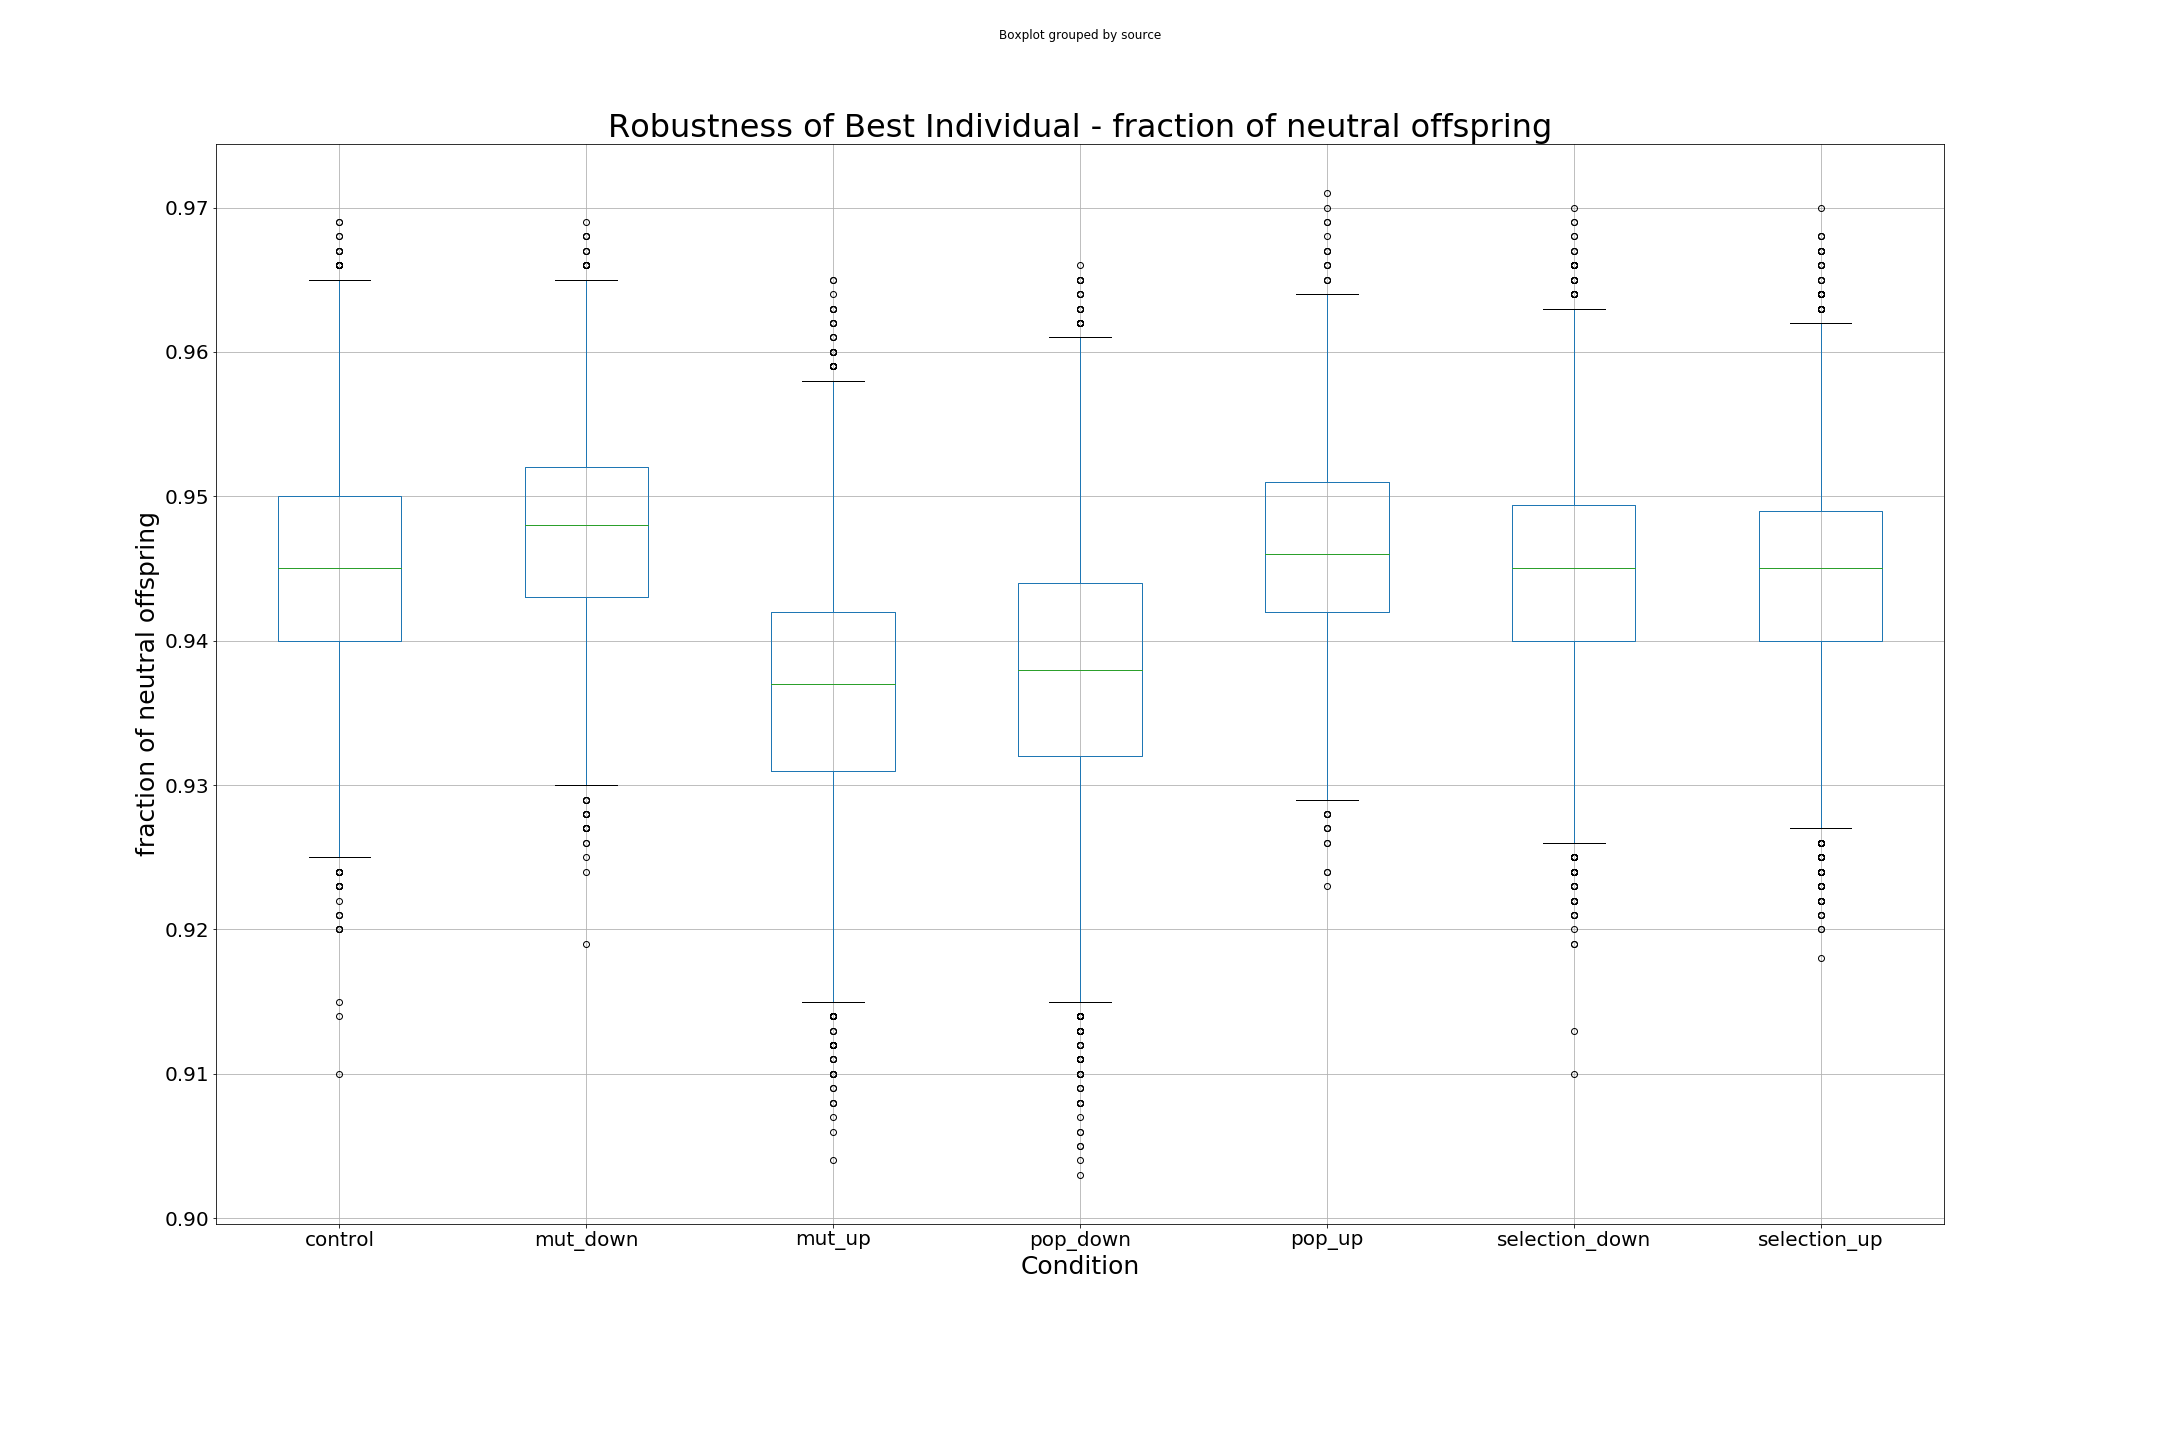
\includegraphics[width=\linewidth]{stat_robustness_best_mean_frac_neutral_offspring}
	\caption[Robustness box and whisker plot]{A box and whisker plot showing the spread of neutral offspring for the best individual at generation 500,000, all conditions. Higher numbers are more robust.}
	\label{fig:mean_robustness_all_conditions}
\end{figure}
The mutation up condition clearly had the largest mean percentage of neutral mutants, at 0.5\%. The full statistics are given in the tables below:

\begin{table}
	\begin{tabular}{|c|c|c|}
		\hline
		\multicolumn{3}{c}{\Large \textbf{Robustness - Rank Sum \& p-values}} \\
		\hline
		& \textbf{rank sum} & \textbf{p-value} \\
		\hline
		\hline
		$\mu_+$ & 16756710.50 & 0.00000000 \\ 
		\hline
		$\mu_-$ & 5741758.00 & 0.00000000 \\ 
		\hline
		$N_-$ & 12493750.00 & 0.00000000 \\ 
		\hline
		$k_+$ & 13580845.50 & 0.00135870 \\ 
		\hline
		$k_-$ & 13925884.00 & 0.00127325 \\ 
		\hline
	\end{tabular}
	\caption[Robustness rank sum \& p-values]{Mean robustness rank sum and p-values for all conditions and all seeds.}
	\label{table:rank_sum_p-values}
\end{table}
\begin{table}[H]
	\begin{tabular}{|c|c|c|c|}
		\hline
		\multicolumn{4}{c}{\Large \textbf{Robustness - means \& standard deviations}} \\
		\hline
		& \textbf{mean} & \textbf{std. dev.} & \textbf{mean's \% change from control} \\
		\hline
		control & 0.944925 & 0.007334 & \textemdash \\ 
		\hline
		$\mu_+$ & 0.936677 & 0.007907 & -0.872870 \\ 
		\hline
		$\mu_-$ & 0.947543 & 0.007066 & 0.276989 \\ 
		\hline
		$k_+$ & 0.944466 & 0.007372 & -0.048598 \\ 
		\hline
		$k_-$ & 0.944516 & 0.007424 & -0.043350 \\ 
		\hline
		$N_-$ & 0.937409 & 0.008846 & -0.795408 \\ 
		\hline
	\end{tabular}
	\caption[Robustness means and standard deviations]{Robustness means and standard deviations for all conditions and all seeds.}
	\label{table:robustness_means_and_std_dev}
\end{table}


\section{Discussion}\label{discussion}

Analogously to Table~\ref{table:experiment_predictions}, the results of the experiments in Table~\ref{table:experiment_results_summary} are summarized below. For each cell, {\color{green} green} indicates that the prediction was confirmed in these experiments and {\color{red}red} indicates that the prediction must be rejected. The predictions for each condition are duplicated here for convenience, with a $+$ indicating a predicted increase and $-$ indicating a predicted decrease over the control condition. 

\begin{table}[H]
	\centering
	\begin{tabular}{|c||c|c|c|c|c|c|}
		\hline
		\multicolumn{7}{|c|}{{\Large \textbf{Experiment Results Summary}}} \\
		\hline \hline
		\multirow{2}{*}{\textbf{Effect On:}} & \multicolumn{6}{c|}{\textbf{Condition}} \\
		\cline{2-7}
		& {\Large$\mu_+$} & {\Large$\mu_-$} & {\Large$k_+$} & {\Large$k_-$} & {\Large$N_+$} & {\Large$N_-$} \\
		\hline 
		Genome Size & \cellcolor{green} $-^{\cite{bradwell2013correlation, carde.2019, marais2008mutation}}$ & \cellcolor{red} $\text{+}^{\cite{bradwell2013correlation, carde.2019, drake1991constant}}$ & \cellcolor{green} $+^{\cite{Batut.2013}}$ & \cellcolor{green} $-^{\cite{Batut.2013}}$ & $-^{\cite{Batut.2014, carde.2019}}$ & \cellcolor{green} $+^{\cite{Batut.2014, carde.2019}}$ \\
		\hline
		Fitness & \cellcolor{green} $+^{\cite{bataillon2000estimation, vahdati2017effect}}$ & \cellcolor{green} $-^{\cite{vahdati2017effect}}$ & \cellcolor{red} $+^{\cite{Batut.2014}}$ & \cellcolor{red} $-^{\cite{Batut.2014}}$ & $+^{\cite{cutter2019primer, vahdati2017effect}} $ & \cellcolor{green} $-^{\cite{cutter2019primer, vahdati2017effect}} $\\
		\hline
		Amount of non-coding DNA & \cellcolor{green} $-^{\cite{Knibbe2007}}$ & \cellcolor{red} $+^{\cite{Knibbe2007}}$ & \cellcolor{green} $+^{\cite{Batut.2013, Knibbe2007}}$ & \cellcolor{green} $-^{\cite{Batut.2013, Knibbe2007}}$ & $-^{\cite{Batut.2013}}$ & \cellcolor{green} $+^{\cite{Batut.2013}}$ \\
		\hline
		Number of genes & \cellcolor{red} $-^{\cite{Knibbe2007}}$ & \cellcolor{green} $+^{\cite{Knibbe2007}}$ &\cellcolor{green} $+^{\cite{Knibbe2007}}$ & \cellcolor{green} $-^{\cite{Knibbe2007}}$ & $-^{\cite{Batut.2014}}$ & \cellcolor{green} $+^{\cite{Batut.2014}}$ \\
		\hline
		Average size of genes & \cellcolor{red} $-^{\cite{Liard.2018}}$ & \cellcolor{green} $+^{\cite{Liard.2018}}$ & \cellcolor{green} $-^{\cite{Batut.2013}}$ & \cellcolor{red}$+^{\cite{Batut.2013}}$ & $-^{\cite{Batut.2014}}$ & \cellcolor{red} $+^{\cite{Batut.2014}}$ \\
		\hline
		Robustness & \cellcolor{green} $-^{\cite{Knibbe2007}}$ &\cellcolor{green} $+^{\cite{Knibbe2007}}$ & \cellcolor{green} $-^{\cite{Batut.2013, Knibbe2007}}$ & \cellcolor{green}$+^{\cite{Batut.2013, Knibbe2007}}$ & $-^{\cite{elena2007effects}}$ & \cellcolor{red} $+^{\cite{elena2007effects}}$ \\
		\hline
		Evolvability &\cellcolor{green} $+^{\cite{Knibbe2007}}$ &\cellcolor{green} $-^{\cite{Knibbe2007}}$ & \cellcolor{red}  $+^{\cite{Batut.2013}}$ & \cellcolor{red} $-^{\cite{Batut.2013}}$ & $-^{\cite{wein2019effect}}$ & \cellcolor{green} $+^{\cite{wein2019effect}}$ \\
		\hline		
	\end{tabular}
	\caption[Experiment result summary]{A summary of whether the experiment results confirmed or denied the hypotheses of Table~\ref{table:experiment_predictions}.  were confirmed ({\color{green}green}) or rejected ({\color{red}red}), along with the predicted results of whether the given result would increase (+) or decrease (-) over the control condition.}
	\label{table:experiment_results_summary}
\end{table}
\subsection{Genome Size}

According to the predictions based on a survey of the literature (as summarized in Table~\ref{table:experiment_predictions}), only the $\mu_+$, $k_-$, and $N_+$ conditions were predicted to lead to a reduced genome. As shown in Figure~\ref{fig:genome_size}, however, although the $\mu_+$ and $k_-$ conditions did end up with a genome size which was noticeably smaller than the control condition, surprisingly $\mu_-$ also experienced a reduction in genome size. %TODO Explain why the u- condution also ended up below control 

Beginning with the $N_-$ condition, recall Table~\ref{table:genome_size_stats_last_50k}. The $N_-$ condition ending up with a genome over 20\% larger than the control condition perfectly illustrates the effects of genetic drift described by Batut et al. with regard to small effective population sizes ($N_e$) \cite{Batut.2014}. The efficacy of selection to remove deleterious mutations and accumulations of non-coding bases is predicted to go down in populations with a smaller effective population size, causing rapid expansion of the genome size. This appears to be exactly what happened here, as Table~\ref{table:non-coding_DNA_mean_and_standard_deviation} shows the amount of non-coding bases greatly expanding, reaching 17.7\% over the control condition. 

Because the wild types began these experiments having evolved for 10 million generations in a static environment, their variability was low and the genome was relatively compact (thanks to the natural streamlining effects of bacterial genomes), and thus their mutational robustness was also low. As described in Liard et al.~\cite{Liard.2018}, however, in the $\mu_+$ condition, an increased mutation rate is expected to boost their mutational robustness by disrupting existing genes and introducing many non-coding bases, which in turn allows purifying selection to overcome the proposed complexity ratchet, finally reducing the genome. In these experiments, however, the robustness scores for the $\mu_+$ condition (see Table~\ref{table:robustness_means_and_std_dev} indicate that increasing the mutation rate did not produce this effect, as the robustness actually went down from the control condition. Nevertheless, in the $\mu_+$ condition, the number of non-coding bases went down (see Table~\ref{table:non-coding_DNA_mean_and_standard_deviation}), the gene density went up (see Table~\ref{table:mean_functional_gene_size_and_std_dev}), and the number of genes overall went down (see Table~\ref{table:number_of_genes_mean_std_dev}). %TODO Expain this!

\subsection{Fitness}
Examining Figure~\ref{fig:mean_fitness_all_seeds}, it quickly becomes apparent that, in the static environment in which the wild type evolved, adding another 500,000 generations on top of the previous 10 million does not much affect the average fitness of the control condition. Small fluctuations occurred due to mutations, insertions, etc. but overall the genotype was quite steady. However, for the $\mu_+$, $\mu_-$, $k_+$, and $N_+$ conditions, a clear trend towards improved fitness may be observed.

More interesting are the $N_-$ and $k_+$ conditions, where by generation 500,000 the average fitness in the whole population declined to 2.76\% and 99.99\% below the control condition respectively (see Table~\ref{table:fitness_means_std_dev}). It seems that with the smaller population size, genetic drift may be more strongly at work in continually increasing the gap between the phenotype and environmental function, as the lack of variety inherent in a smaller population causes a cascade of increasingly deleterious consequences.
 
It has been postulated that perhaps gene loss may be selected for in order to increase the overall fitness of an organism by removing the added cost of the superfluous genes~\cite{koskiniemi2012}. These results generally agree with this hypothesis, though the results show that, in addition to the general accumulation of non-coding DNA across all conditions (Figure~\ref{fig:mean_non-coding_DNA}), which would theoretically have a higher fitness cost, the number of genes actually \textit{increased} slightly for each condition, except for $k_-$. Likewise, fitness overall went \textit{up} as the number of genes increased (except for $N_-$). Lastly, decreasing the selection pressure resulted in the highest overall mean fitness by a wide margin (Table~\ref{table:fitness_means_std_dev}). In Aevol, non-coding DNA is not directly associated with a fitness cost, so this may not fully explain the circumstances.  

\subsection{Functional Genes}
Regarding the $N_-$ condition, comparing this with the results of Batut et al. and their work with \textit{Buchnera aphidicola} (see Section~\ref{related_work}), it may be possible that gene loss is occurring because of the smaller effective population size clicking down Muller's ratchet. This does not seem to be what is happening in these experiments either, however. Though mean fitness of the $N_-$ condition did greatly decline (see Figure~\ref{fig:mean_fitness_plot}), the $N_-$ condition also saw the largest accumulation of non-coding DNA (see Figure~\ref{fig:mean_non-coding_DNA}) and the second-highest level of evolvability (see Table~\ref{table:mean_std_dev_evolvability}), which should theoretically have lead to an easier time of overcoming the ratchet. On the other hand, the number of functional genes stayed more or less the same as all of the other conditions, and the accumulated number of non-functional genes (pseudogenes) of the $N_-$ condition was the largest (see Figure~\ref{fig:mean_num_non-functional_genes}). These two factors together suggest that there almost certainly was some loss of fitness through pseudogenization; perhaps with more time, the pseudogenes would also have been lost.

Recall the work of Liard et al.\cite{Liard.2018} as discussed in Section~\ref{related_work}, in which the proposed ``complexity ratchet'' was overcome by increasing the mutation rate. Their work was quite successful in overcoming this ratchet, but in the experiments of this thesis, both the number of genes and the average size of the genes increased. One possible explanation for this is that, in their work, their increased mutation rate $\mu_+$ was set to $1e^{-3}$.  By contrast, even the elevated mutation rate used here, $\mu_+$, was just $4e^{-7}$, which is $\frac{1}{4}*e^4 \approx 13.65$ times lower than their highest mutation rate. Perhaps an even higher mutation rate would be sufficient to overcome the power of selection and reduce the genome further. 

\subsection{Robustness \& Evolvability}
%The robustness results indicate that the stable environment is not encouraging much differentiation between the different conditions.  The average difference in robustness between any of the conditions and the control condition was only 0.002803, i.e. only 0.28\%. Robustness does not seem to be selected for in any of the conditions. 
%
%The reduced evolvability again seems to be playing a role, as the 



%TODO Perform another experiment with a much higher mutation rate: 1e-3 for 100k generations?

